\chapter{Classical Probability}\cite{joeblitztein}

Whatever we learnt in the previous chapter, will be useful in the next chapter. In this chapter, I want to recap all the basic concepts of probability we have studied previously and at the end demonstrate - why we need a better, a more rigorous framework, for the probability theory. \\

Just as a point is not defined in elementary geometry, probability theory begins with two entities that are not defined. These undefined entities are a \textit{Random Experiment} and its \textit{Outcome}. These two concepts are to be understood intuitively, as suggested by their respective English meanings. We use these undefined terms to define other entities. \\

So, let's begin!

\section{Probability and Counting}

The first concept in the probability theory is the \textit{sample space} and the \textit{event}. 

\begin{definition}
    The sample space, often denoted by \( S \), is the set of all possible outcomes of a random experiment. Formally, if an experiment can result in one of \( n \) distinct outcomes, the sample space is the set containing all these outcomes.

\[
S = \{ \omega_1, \omega_2, \dots, \omega_n \}
\]
\end{definition}


\textit{Example:} For a single coin flip, the sample space is:

\[
S = \{ \text{Heads}, \text{Tails} \}
\]

\begin{definition}
    An event is a subset of the sample space. It represents one or more outcomes that may occur as a result of the experiment. Formally, if \( A \) is an event, then \( A \subseteq S \).
\end{definition}

\textit{Example:} If we roll a die, the sample space is \( S = \{1, 2, 3, 4, 5, 6\} \). An event could be rolling an even number:

\[
A = \{2, 4, 6\}
\]

An event \( A \) occurs if the outcome of the experiment is one of the elements of the subset \( A \). Mathematically, this means that if the outcome of the experiment is \( \omega \), we say the event \( A \) has occurred if \( \omega \in A \). \\

\textit{Example:} If we roll a die and the outcome is 4, the event \( A = \{2, 4, 6\} \) (rolling an even number) has occurred because \( 4 \in A \). \\

The probability of an event occuring is given by the \textit{naive definition of the probability.} The definition is called \textit{naive} because it has some gaps in it, but it works fairly well in many cases and only errs when dealing with \textit{infinitely big sample spaces}. As in real world, most of the experiments have finite number of outcomes - we can progress our theory for now and fix it later. 

\begin{definition}
    If all outcomes in the sample space \( S \) are equally likely, the probability of an event \( A \), denoted by \( P(A) \), is given by:

\[
P(A) = \frac{|A|}{|S|}
\]

where \( |A| \) is the number of outcomes in the event \( A \), and \( |S| \) is the total number of outcomes in the sample space \( S \).
\end{definition}

\textit{Example:} In a fair six-sided die roll, the probability of rolling an even number (event \( A = \{2, 4, 6\} \)) is:

\[
P(A) = \frac{|A|}{|S|} = \frac{3}{6} = \frac{1}{2}
\]

\textit{\textbf{Spoiler Alert!}} What happens when the outcomes are not exactly likely? You can imagine how flawed the argument sounds when I ask \textit{What's the probability of life on Mars?} and someone replies that there are two possibilities - either there is a life or not; hence the probability of life on Mars is 50\%. So now you are already seeing why this definition is called \textit{naive}. The theory that fixes this or improves our understanding of probability is the \textit{Bayesian Theory!} There is a lot of prerequisites that we have to cover before we touch that!

\subsection{Counting}

\begin{definition}
    If an event can occur in \( n_1 \) ways and another mutually exclusive event can occur in \( n_2 \) ways, the total number of ways either of the two events can occur is:
\[
n_1 + n_2
\]
\end{definition}

This rule applies when we are selecting from two or more disjoint sets. \\

\textit{Example:} If you can choose a red shirt in 3 ways and a blue shirt in 5 ways, and you can only choose one shirt, the total number of choices is:
\[
3 + 5 = 8
\]

\begin{definition}
    If a procedure can be broken down into two stages, where the first stage can occur in \( n_1 \) ways and for each of these the second stage can occur in \( n_2 \) ways, the total number of ways to perform the procedure is:
\[
n_1 \times n_2
\]
\end{definition}

This rule applies when events are independent and occur sequentially. \\

\textit{Example:} If you have 3 shirts and 2 pants to choose from, the total number of ways to select an outfit is:
\[
3 \times 2 = 6
\]

\begin{definition}
    A permutation is an arrangement of \( k \) objects from \( n \) distinct objects where the order of selection matters. The number of permutations is given by:
\[
P(n, k) = \frac{n!}{(n-k)!}
\]
\end{definition}

\textit{Example:} The number of ways to arrange 3 students out of 5 is:
\[
P(5, 3) = \frac{5!}{(5-3)!} = 5 \times 4 \times 3 = 60
\]

\begin{definition}
    A combination is a selection of \( k \) objects from \( n \) distinct objects where the order of selection does not matter. The number of combinations is given by:
\[
C(n, k) = \binom{n}{k} = \frac{n!}{k!(n-k)!}
\]
\end{definition}

\textit{Example:} The number of ways to choose 3 students out of 5 is:
\[
C(5, 3) = \binom{5}{3} = \frac{5!}{3!(5-3)!} = \frac{5 \times 4 \times 3}{3 \times 2 \times 1} = 10
\]

\subsubsection{Sampling Table}

We can summarize the different ways of selecting items using the following 2x2 table, which distinguishes between sampling with and without replacement, and whether the order of selection matters or not.

\[
\begin{array}{|c|c|c|}
\hline
\textbf{Selection Criteria} & \textbf{With Replacement} & \textbf{Without Replacement} \\
\hline
\text{Order Matters} & n^k & \frac{n!}{(n-k)!} \\
\hline
\text{Order Doesn't Matter} & \binom{n+k-1}{k} & \binom{n}{k} \\
\hline
\end{array}
\]
\vspace{5pt}

\textbf{Scenario:} Imagine you're visiting a candy store with 5 different types of candies. You're interested in selecting some candies, and we will explore four different ways you might select these candies based on the two criteria: 
\begin{itemize}
    \item whether you put back the candy after picking (with or without replacement)
    \item whether the order in which you pick the candies matters
\end{itemize} 

\subsubsection*{With Replacement, Order Matters}
Let's say you want to select 3 candies one by one, and every time you pick a candy, you put it back into the box before picking the next one. Also, you care about the order in which the candies are picked (perhaps because you are arranging them in a special pattern). \\

\textbf{Story Proof:} The first candy you pick can be any of the 5 types. Since you put the candy back, when you pick the second candy, you again have 5 choices. For the third candy, you once again have 5 choices, because the previous candies were returned. Thus, for each of the 3 choices, there are 5 options, resulting in \( 5 \times 5 \times 5 = 5^3 = 125 \) different possible ways to select the candies.

\subsubsection*{Without Replacement, Order Matters}

Now, imagine you're selecting 3 candies, but this time after selecting a candy, you do \textbf{not} put it back into the box. You still care about the order of selection. \\

\textbf{Story Proof:} For the first candy, you have 5 choices, as all candies are available. After picking the first candy, you're left with 4 candies to choose from for the second selection. Once the second candy is selected, only 3 candies remain for the third selection. Therefore, the total number of ways to arrange these candies is \( 5 \times 4 \times 3 = 60 \). 

\subsubsection*{With Replacement, Order Doesn't Matter}

Let's change the scenario. Now, you are still selecting 3 candies, but every time you pick a candy, you put it back into the box, and this time, you don’t care about the order in which you pick them.\\

\textbf{Story Proof:} You are choosing 3 candies, and since you put the candy back after each selection, it’s possible to select the same candy more than once. However, because the order doesn’t matter, we don't treat "Red, Green, Blue" as different from "Blue, Green, Red." To count how many different groups of candies you can pick, we think of it as a combination with repetition. The formula to calculate this is \( \binom{n+k-1}{k} \), where \( n \) is the number of candy types, and \( k \) is the number of candies you’re choosing. In this case, there are \( \binom{5+3-1}{3} = \binom{7}{3} = 35 \) different combinations of candies.

\subsubsection*{Without Replacement, Order Doesn't Matter}

Finally, let’s consider the case where you’re selecting 3 candies, but you don’t put the candies back after picking, and you don’t care about the order in which they are picked.\\

\textbf{Story Proof:} You are choosing 3 candies from the 5 available types, but once you pick a candy, you don't replace it. Since the order doesn’t matter, we only care about which candies were chosen, not the sequence of selection. To count how many different groups of candies you can pick, we use combinations. The number of ways to choose 3 candies from 5 without caring about the order is given by \( \binom{5}{3} = 10 \). \\

There are some more story proofs!

\subsubsection{Choosing the complement}

For nonnegative integers \(n\) and \(k\) with \(k \leq n\), we have:
\[
\binom{n}{k} = \binom{n}{n-k}.
\]

\textbf{Story Proof:} Consider selecting a committee of size \(k\) from \(n\) people. You can either choose \(k\) people to be on the committee or equivalently choose the \(n-k\) people who will \textit{not} be on the committee. Both methods count the same outcome, so the two binomial coefficients are equal.

\subsubsection{The Team Captain}

For positive integers \(n\) and \(k\) with \(k \leq n\), we have:
\[
\binom{n}{k} = k \cdot \binom{n-1}{k-1}.
\]

\textbf{Story Proof:} Suppose we are choosing a team of \(k\) people from \(n\) individuals, one of whom will be the captain. First, choose the team captain, then select the remaining \(k-1\) members from the remaining \(n-1\) individuals. Alternatively, select the \(k\)-member team first, then choose one of the \(k\) members to be the captain.

\subsubsection{Vandermonde's Identity}

Vandermonde's identity states:
\[
\binom{m+n}{k} = \sum_{j=0}^{k} \binom{m}{j} \binom{n}{k-j}.
\]

\textbf{Story Proof:} Consider choosing a committee of \(k\) members from a group of \(m\) men and \(n\) women. If the committee has \(j\) men, then the remaining \(k-j\) members must be women. The right-hand side sums over all possible values of \(j\), showing different ways to form the committee.

\subsubsection{Partnerships}

We show:
\[
\frac{(2n)!}{2^n \cdot n!} = (2n-1)(2n-3) \cdots 3 \cdot 1.
\]

\textbf{Story Proof:} Consider breaking \(2n\) people into \(n\) partnerships. First, line them up, and pair the first two, the next two, and so on. This overcounts by \(n! \cdot 2^n\) because the order of pairs and the order within pairs doesn't matter. Alternatively, pick the first partner from \(2n-1\), the next from \(2n-3\), and so on, yielding the right-hand side.

\subsection{Classical Problems on Probability}

\subsubsection{The Birthday Problem}

\textit{What is the minimum number of people required to have a 50\% chance of at least two people sharing the same birthday?} \\

The total number of ways to assign birthdays to \(n\) people (assuming 365 possible days) is \(365^n\). The probability that no two people share the same birthday can be computed by considering that the first person can have any of the 365 days, the second person can have 364 remaining days, the third person 363, and so on. The probability that all \(n\) people have distinct birthdays is:

\[
P(\text{no shared birthdays}) = \frac{365}{365} \cdot \frac{364}{365} \cdot \frac{363}{365} \cdots \frac{365-n+1}{365}.
\]

The probability of at least one birthday clash is:
\[
P(\text{at least one shared birthday}) = 1 - P(\text{no shared birthdays}).
\]

We seek the smallest \(n\) such that \(P(\text{at least one shared birthday}) \geq 0.5\). This gives the inequality:

\[
1 - \frac{365}{365} \cdot \frac{364}{365} \cdot \frac{363}{365} \cdots \geq 0.5.
\]

Solving numerically, we find that \(n = 23\) gives a probability slightly greater than 0.5. \\

With just 23 people, the probability of at least two people sharing the same birthday is about 50\%. This counterintuitive result occurs because with 23 people, there are many possible pairs, and the chance of any two people sharing a birthday grows rapidly as the number of people increases.

\subsubsection{Newton-Pepys Problem}

\textit{Which event has the highest probability?
\begin{itemize}
    \item A: At least one 6 appears when 6 dice are rolled.
    \item B: At least two 6's appear when 12 dice are rolled.
    \item C: At least three 6's appear when 18 dice are rolled.
\end{itemize}}

The probability of getting at least \(k\) sixes when rolling \(n\) dice can be computed using the binomial distribution. For each die, the probability of rolling a 6 is \(p = \frac{1}{6}\), and the probability of not rolling a 6 is \(\frac{5}{6}\). The probability of getting exactly \(k\) sixes in \(n\) dice is:

\[
P(\text{exactly } k \text{ sixes}) = \binom{n}{k} p^k (1-p)^{n-k}.
\]

To calculate the probability of getting at least \(k\) sixes, we compute:

\[
P(\text{at least } k \text{ sixes}) = 1 - P(\text{fewer than } k \text{ sixes}).
\]

For each case:
\begin{itemize}
    \item For \(n = 6\), \(k = 1\):
    \[
    P(\text{at least one 6}) = 1 - \left(\frac{5}{6}\right)^6 \approx 0.6651.
    \]
    \item For \(n = 12\), \(k = 2\):
    \[
    P(\text{at least two 6's}) = 1 - \sum_{i=0}^{1} \binom{12}{i} \left(\frac{1}{6}\right)^i \left(\frac{5}{6}\right)^{12-i} \approx 0.6187.
    \]
    \item For \(n = 18\), \(k = 3\):
    \[
    P(\text{at least three 6's}) = 1 - \sum_{i=0}^{2} \binom{18}{i} \left(\frac{1}{6}\right)^i \left(\frac{5}{6}\right)^{18-i} \approx 0.5973.
    \]
\end{itemize}

\subsubsection{De Montmort's Matching Problem}

\textit{Consider a deck of \(n\) cards labeled from 1 to \(n\). You flip over the cards one by one, saying the numbers 1 through \(n\) as you do. You win if, at some point, the number you say matches the number on the card. What is the probability of winning?} \\

Let \(A_i\) be the event that the \(i\)-th card is in position \(i\) (i.e., a match for card \(i\)). We are interested in the probability of the union of these events:
\[
P\left(\bigcup_{i=1}^n A_i\right),
\]
which is the probability that at least one card is in its correct position. To calculate this, we will use the inclusion-exclusion principle. \\

The inclusion-exclusion formula for the union of \(n\) events is:
\begin{align*}
    P\left(\bigcup_{i=1}^n A_i\right) & = \sum_{i=1}^n P(A_i) - \sum_{1 \leq i < j \leq n} P(A_i \cap A_j)  + \sum_{1 \leq i < j < k \leq n} P(A_i \cap A_j \cap A_k) \\
    & \quad - \cdots + (-1)^{n+1} P(A_1 \cap A_2 \cap \cdots \cap A_n).
    \end{align*}
    
Since the problem is symmetric, the probabilities of individual intersections of events \(A_i\) are the same for any \(i\), and the expression simplifies considerably.\\

The probability that the \(i\)-th card is in the \(i\)-th position (i.e., a match) is:
\[
P(A_i) = \frac{1}{n}.
\]
This is because there are \(n!\) possible orderings of the deck, and in \((n-1)!\) of them, card \(i\) is in position \(i\) (with the remaining \(n-1\) cards arranged freely).\\

Next, consider the probability that two specific cards, \(i\) and \(j\), are both in their correct positions. If both cards \(i\) and \(j\) are fixed in positions \(i\) and \(j\), there are \((n-2)!\) favorable arrangements for the remaining \(n-2\) cards, so:
\[
P(A_i \cap A_j) = \frac{(n-2)!}{n!} = \frac{1}{n(n-1)}.
\]

Similarly, the probability that three specific cards, \(i\), \(j\), and \(k\), are all in their correct positions is:
\[
P(A_i \cap A_j \cap A_k) = \frac{(n-3)!}{n!} = \frac{1}{n(n-1)(n-2)}.
\]

Thus, the inclusion-exclusion formula for the union becomes:
\[
P\left(\bigcup_{i=1}^n A_i\right) = \sum_{i=1}^n \frac{1}{n} - \sum_{1 \leq i < j \leq n} \frac{1}{n(n-1)} + \sum_{1 \leq i < j < k \leq n} \frac{1}{n(n-1)(n-2)} - \cdots + (-1)^{n+1} \frac{1}{n!}.
\]

This simplifies to:
\[
P\left(\bigcup_{i=1}^n A_i\right) = 1 - \frac{1}{2!} + \frac{1}{3!} - \cdots + \frac{(-1)^{n+1}}{n!}.
\]

This is the partial sum of the Taylor series expansion of \(e^{-1}\), which is given by:
\[
e^{-1} = 1 - \frac{1}{1!} + \frac{1}{2!} - \frac{1}{3!} + \cdots.
\]

Thus, for large \(n\), the probability of winning (i.e., having at least one match) is approximately:
\[
P\left(\bigcup_{i=1}^n A_i\right) \approx 1 - \frac{1}{e}.
\]

Since \(1 - \frac{1}{e} \approx 0.6321\), the probability of winning the game is about 63.2\%.


\section{Conditional Probability}

Conditional probability is a fundamental concept in probability theory that allows us to update our beliefs about an event based on new information or evidence. It helps in understanding how the probability of one event changes in the presence of another event. This concept is particularly useful in various fields such as statistics, machine learning, and decision-making, where we often deal with uncertain events and seek to refine our predictions.

\begin{definition}  
If \( A \) and \( B \) are events with \( P(B) > 0 \), then the conditional probability of \( A \) given \( B \), denoted by \( P(A|B) \), is defined as:

\[
P(A|B) = \frac{P(A \cap B)}{P(B)}.
\]
\end{definition}

In this definition, \( A \) is the event whose uncertainty we want to update, and \( B \) is the evidence we observe (or want to treat as given). We refer to \( P(A) \) as the prior probability of \( A \) and \( P(A|B) \) as the posterior probability of \( A \). The term "prior" indicates our initial belief about the event before incorporating the new evidence, while "posterior" reflects our updated belief after taking the evidence into account.\\

Similarly, we can express the conditional probability of event \( B \) given event \( A \) as:

\[
P(B|A) = \frac{P(A \cap B)}{P(A)} \quad \text{for } P(A) > 0.
\]

From these two definitions, we can express \( P(A \cap B) \) in two different ways:
\[
P(A \cap B) = P(A|B) \cdot P(B)
\]
\[
P(A \cap B) = P(B|A) \cdot P(A)
\]

Since both expressions represent the same quantity, we can set them equal to each other:

\[
P(A|B) \cdot P(B) = P(B|A) \cdot P(A)
\]

Now, to isolate \( P(A|B) \), we divide both sides by \( P(B) \) (assuming \( P(B) > 0 \)):

\[
P(A|B) = \frac{P(B|A) \cdot P(A)}{P(B)}
\]

This is the formulation of \textbf{Bayes' theorem}, which expresses the conditional probability of event \( A \) given event \( B \) in terms of the conditional probability of event \( B \) given event \( A \), the prior probability of \( A \), and the marginal probability of \( B \):

\[
P(A|B) = \frac{P(B|A) \cdot P(A)}{P(B)}
\]

\begin{theorem}
    If \( A \) and \( B \) are events such that \( P(B) > 0 \), Bayes' theorem states that:

\[
P(A|B) = \frac{P(B|A) \cdot P(A)}{P(B)}
\]
\end{theorem}

\textbf{Explanation of the Terms:}

\begin{itemize}
    \item \( P(A|B) \): The posterior probability of \( A \) given \( B \), which reflects our updated belief about \( A \) after observing \( B \).
    \item \( P(B|A) \): The likelihood, or the probability of observing \( B \) given that \( A \) is true. This measures how well \( A \) explains the observed evidence \( B \)
    \item \( P(A) \): The prior probability of \( A \), representing our initial belief about \( A \) before considering the evidence \( B \).
    \item \( P(B) \): The marginal probability of \( B \), which can be computed using the law of total probability, as described in the next theorem.
\end{itemize}

\textbf{Intuition Behind Bayes' Theorem:}\\

Bayes' theorem allows us to revise our beliefs in light of new evidence. For example, suppose we want to determine the probability that a patient has a certain disease (event \( A \)) given that they tested positive for it (event \( B \)). Using Bayes' theorem, we can incorporate the accuracy of the test (the likelihood \( P(B|A) \)), our initial belief about the prevalence of the disease (the prior \( P(A) \)), and the overall rate of positive tests (the marginal \( P(B) \)) to arrive at a more informed estimate of the probability that the patient actually has the disease.

\begin{theorem}
    The law of total probability provides a way to compute the total probability of an event based on a partition of the sample space. It states that if \( B_1, B_2, \ldots, B_n \) are mutually exclusive events that form a complete partition of the sample space, then for any event \( A \):

\[
P(A) = \sum_{i=1}^n P(A|B_i) \cdot P(B_i).
\]
\end{theorem}

\textbf{Explanation of the Terms:}

\begin{itemize}
    \item \( P(A) \): The total probability of the event \( A \).
    \item \( P(A|B_i) \): The conditional probability of \( A \) given that the event \( B_i \) has occurred.
    \item  \( P(B_i) \): The probability of each partition event \( B_i \).
\end{itemize}

\textbf{Intuition Behind Law of Total Probability:}\\

The law of total probability helps us compute the probability of an event by considering all possible scenarios (the partition \( B_i \)) that could lead to that event. For instance, if we want to determine the probability that it will rain tomorrow (event \( A \)), we might partition the sample space based on different weather conditions (e.g., sunny, cloudy, or stormy). By calculating the probability of rain under each condition and weighting these probabilities by the likelihood of each condition occurring, we can obtain the overall probability of rain.

\subsection{Classical Problems on Conditional Probability}

\subsubsection{Which coin was tossed?}

\textit{You have one fair coin and one biased coin that lands Heads with probability \( \frac{3}{4} \). You pick one of the coins at random and flip it three times. It lands Heads all three times. Given this information, what is the probability that the coin you picked is the fair one?}\\

Let \( A \) be the event that the chosen coin lands Heads three times, and let \( F \) be the event that we picked the fair coin. We are interested in \( P(F | A) \), but it is easier to find \( P(A | F) \) and \( P(A | F^c) \) since it helps to know which coin we have; this suggests using Bayes’ rule and the law of total probability. Doing so, we have

\[
P(F | A) = \frac{P(A | F) P(F)}{P(A)}.
\]

By the law of total probability, 

\[
P(A) = P(A | F) P(F) + P(A | F^c) P(F^c).
\]

Given that \( P(F) = P(F^c) = \frac{1}{2} \), we can compute:

\[
P(A | F) = \left(\frac{1}{2}\right)^3 = \frac{1}{8},
\]

\[
P(A | F^c) = \left(\frac{3}{4}\right)^3 = \frac{27}{64}.
\]

Thus, we have

\[
P(A) = P(A | F) P(F) + P(A | F^c) P(F^c) = \left(\frac{1}{8} \cdot \frac{1}{2}\right) + \left(\frac{27}{64} \cdot \frac{1}{2}\right) = \frac{1}{16} + \frac{27}{128}.
\]

Calculating this gives:

\[
P(A) = \frac{8}{128} + \frac{27}{128} = \frac{35}{128}.
\]

Now, substituting back into Bayes' theorem:

\[
P(F | A) = \frac{P(A | F) P(F)}{P(A)} = \frac{\left(\frac{1}{8}\right) \cdot \left(\frac{1}{2}\right)}{\frac{35}{128}} = \frac{\frac{1}{16}}{\frac{35}{128}} = \frac{128}{560} \approx 0.23.
\]

Before flipping the coin, we thought we were equally likely to have picked the fair coin as the biased coin: \( P(F) = P(F^c) = \frac{1}{2} \). Upon observing three Heads, however, it becomes more likely that we’ve chosen the biased coin than the fair coin, so \( P(F | A) \) is only about \( 0.23 \). \\

\textbf{Prior vs. Posterior:} It would not be correct in the calculation in the above example to say after the first step, \( P(A) = 1 \) because we know \( A \) happened. It is true that \( P(A|A) = 1 \), but \( P(A) \) is the prior probability of \( A \) and \( P(F) \) is the prior probability of \( F \)—both are the probabilities before we observe any data in the experiment. These must not be confused with posterior probabilities conditional on the evidence \( A \).

\subsubsection{Testing a rare disease}

Consider a rare disease that affects \(1\%\) of a population. A diagnostic test is available for this disease, which has the following characteristics:
\begin{itemize}
    \item The probability of testing positive if the person has the disease (true positive rate) is \(P(\text{Positive} | \text{Disease}) = 0.95\).
    \item The probability of testing positive if the person does not have the disease (false positive rate) is \(P(\text{Positive} | \text{No Disease}) = 0.10\).
\end{itemize}

We want to find the probability that a person has the disease given that they tested positive for the disease, denoted as \(P(\text{Disease} | \text{Positive})\).\\

Using Bayes' theorem, we can express the conditional probability as follows:

\[
P(\text{Disease} | \text{Positive}) = \frac{P(\text{Positive} | \text{Disease}) \cdot P(\text{Disease})}{P(\text{Positive})}.
\]

To compute this, we need to determine \(P(\text{Positive})\) using the law of total probability:

\[
P(\text{Positive}) = P(\text{Positive} | \text{Disease}) \cdot P(\text{Disease}) + P(\text{Positive} | \text{No Disease}) \cdot P(\text{No Disease}).
\]

Given that \(P(\text{Disease}) = 0.01\) and \(P(\text{No Disease}) = 1 - P(\text{Disease}) = 0.99\), we can substitute the values:

\[
P(\text{Positive}) = (0.95 \cdot 0.01) + (0.10 \cdot 0.99) = 0.0095 + 0.099 = 0.1085.
\]

Now we can calculate \(P(\text{Disease} | \text{Positive})\):

\[
P(\text{Disease} | \text{Positive}) = \frac{0.95 \cdot 0.01}{0.1085} = \frac{0.0095}{0.1085} \approx 0.0875.
\]

Thus, the probability that a person has the disease given that they tested positive is approximately \(8.75\%\).\\

Now, let's consider the situation where the same person tests positive a second time. We need to update our previous result using Bayes' theorem again. \\

Let \(B\) represent the event that the person tests positive again. We want to find \(P(\text{Disease} | B \cap \text{Positive})\). \\

Using the law of total probability, we find \(P(B | \text{Disease})\) and \(P(B | \text{No Disease})\): 

\[
P(B | \text{Disease}) = P(\text{Positive} | \text{Disease}) = 0.95,
\]
\[
P(B | \text{No Disease}) = P(\text{Positive} | \text{No Disease}) = 0.10.
\]

Now, we can calculate the probability of a second positive test:

\[
P(B) = P(B | \text{Disease}) \cdot P(\text{Disease} | \text{Positive}) + P(B | \text{No Disease}) \cdot P(\text{No Disease} | \text{Positive}).
\]

Calculating \(P(\text{No Disease} | \text{Positive})\):

\[
P(\text{No Disease} | \text{Positive}) = 1 - P(\text{Disease} | \text{Positive}) \approx 1 - 0.0875 = 0.9125.
\]

Substituting in the values:

\[
P(B) = (0.95 \cdot 0.0875) + (0.10 \cdot 0.9125) \approx 0.083125 + 0.09125 = 0.174375.
\]

Now we can find \(P(\text{Disease} | B)\):

\[
P(\text{Disease} | B) = \frac{P(B | \text{Disease}) \cdot P(\text{Disease} | \text{Positive})}{P(B)} = \frac{0.95 \cdot 0.0875}{0.174375} \approx \frac{0.083125}{0.174375} \approx 0.477.
\]

Thus, after a second positive test, the updated probability that the person has the disease is approximately \(47.7\%\).\\

This illustrates how Bayes' theorem allows us to update our beliefs about the probability of having a disease as new information becomes available. Initially, the probability was low due to the rarity of the disease, but successive positive test results significantly increased the probability of having the disease.

\subsubsection{Monty-Hall Problem}

The Monty Hall problem is a famous probability puzzle based on a game show scenario. The setup is as follows: \\

A contestant is presented with three doors: Behind one door is a car (the prize), and behind the other two doors are goats (non-prizes). The contestant picks one door, say Door 1. The host, Monty Hall, who knows what is behind each door, opens another door (say Door 3), revealing a goat. The contestant is then given a choice: stick with their original choice (Door 1) or switch to the remaining closed door (Door 2).\\

We want to determine whether the contestant should stick with their original choice or switch doors to maximize their chances of winning the car.\\

Let's define the events:

\begin{itemize}
    \item Let \(C_i\) be the event that the car is behind Door \(i\) for \(i = 1, 2, 3\).
    \item Let \(D\) be the event that Monty opens Door 3.
\end{itemize}

We want to find the conditional probability \(P(C_1 | D)\), the probability that the car is behind Door 1 given that Monty opens Door 3.\\

According to Bayes' theorem, we have:

\[
P(C_1 | D) = \frac{P(D | C_1) \cdot P(C_1)}{P(D)}.
\]


1. \textit{Prior Probability}:\\

   The probability that the car is behind any specific door is equal:

   \[
   P(C_1) = P(C_2) = P(C_3) = \frac{1}{3}.
   \]

2. \textit{Likelihood}:\\

   We need to find \(P(D | C_1)\), the probability that Monty opens Door 3 given that the car is behind Door 1. If the car is behind Door 1, Monty can open either Door 2 or Door 3 (both have goats). Thus, he will open Door 3 with probability \(1/2\):

   \[
   P(D | C_1) = \frac{1}{2}.
   \]

   Now, we calculate \(P(D | C_2)\) and \(P(D | C_3)\):\\

   (a) If the car is behind Door 2, Monty must open Door 3 (the only door he can open that reveals a goat):

   \[
   P(D | C_2) = 1.
   \]

   (b) If the car is behind Door 3, Monty cannot open Door 3, so:\\

   \[
   P(D | C_3) = 0.
   \]

3. \textit{Total Probability}:\\

   Now we need to calculate \(P(D)\):

   \[
   P(D) = P(D | C_1) \cdot P(C_1) + P(D | C_2) \cdot P(C_2) + P(D | C_3) \cdot P(C_3).
   \]

   Substituting the values we found:

   \[
   P(D) = \left(\frac{1}{2} \cdot \frac{1}{3}\right) + (1 \cdot \frac{1}{3}) + (0 \cdot \frac{1}{3}) = \frac{1}{6} + \frac{1}{3} = \frac{1}{6} + \frac{2}{6} = \frac{3}{6} = \frac{1}{2}.
   \]

Now we can use Bayes' theorem:

\[
P(C_1 | D) = \frac{P(D | C_1) \cdot P(C_1)}{P(D)} = \frac{\left(\frac{1}{2}\right) \cdot \left(\frac{1}{3}\right)}{\frac{1}{2}} = \frac{\frac{1}{6}}{\frac{1}{2}} = \frac{1}{3}.
\]

Thus, \(P(C_1 | D) = \frac{1}{3}\).

Next, we calculate \(P(C_2 | D)\):

\[
P(C_2 | D) = \frac{P(D | C_2) \cdot P(C_2)}{P(D)} = \frac{1 \cdot \frac{1}{3}}{\frac{1}{2}} = \frac{\frac{1}{3}}{\frac{1}{2}} = \frac{2}{3}.
\]

The probabilities are:

\[
P(C_1 | D) = \frac{1}{3}, \quad P(C_2 | D) = \frac{2}{3}.
\]

This means that if the contestant switches to Door 2 after Monty reveals Door 3, their chances of winning the car increase to \( \frac{2}{3} \). Therefore, it is advantageous for the contestant to switch doors, rather than stick with their original choice.\\

The intuitive reasoning behind this is: Monty knows where the car is and always opens a door with a goat behind it. This action provides additional information. If your initial choice was wrong (which happens 2/3 of the time), Monty has only one option to reveal a goat. If you switch after Monty reveals a goat, you effectively take advantage of the higher probability that the car is behind one of the doors you didn't initially choose. By switching, you win the car 2/3 of the time.

\subsubsection{Gambler's Ruin Problem}

Consider a gambler (Player 1) who starts with \( m \) dollars and plays a game against another player (Player 2) who has \( N - m \) dollars. Player 1 wins each round with a probability \( p \) and loses with probability \( q = 1 - p \). We aim to find the probability \( P(m) \) that Player 1 eventually reaches \( N \) dollars before going broke.\\

Let \( P(m) \) be the probability of reaching \( N \) dollars starting with \( m \) dollars. The boundary conditions are:
\begin{align*}
P(0) &= 0 \quad (\text{if Player 1 has no money, they cannot win}) \\
P(N) &= 1 \quad (\text{if Player 1 has } N \text{ dollars, they have won})
\end{align*}

Using the law of total probability, we can express the probability recursively:
\[
P(m) = p P(m+1) + q P(m-1)
\]

Rearranging the above equation gives:
\[
p P(m+1) - P(m) + q P(m-1) = 0
\]
This is a second-order linear difference equation. The general solution has the form:
\[
P(m) = A + B r^m
\]
where \( r = \frac{q}{p} \) and \( A \) and \( B \) are constants determined by the boundary conditions. \\

1. Using \( P(0) = 0 \):
   \[
   0 = A + B r^0 \implies A + B = 0 \implies A = -B
   \]

2. Using \( P(N) = 1 \):
   \[
   1 = -B + B r^N \implies 1 = B (r^N - 1) \implies B = \frac{1}{r^N - 1}
   \]
   Thus, substituting \( A \):
   \[
   A = -B = -\frac{1}{r^N - 1}
   \]

We have:
\[
P(m) = -\frac{1}{r^N - 1} + \frac{1}{r^N - 1} r^m = \frac{r^m - 1}{r^N - 1}
\]
Substituting \( r = \frac{q}{p} \):
\[
P(m) = \frac{\left( \frac{q}{p} \right)^m - 1}{\left( \frac{q}{p} \right)^N - 1}
\]

In the special case where the game is fair, we have \( p = \frac{1}{2} \) and \( q = \frac{1}{2} \). Substituting these values into our probability expression, we find:
\[
r = \frac{q}{p} = \frac{\frac{1}{2}}{\frac{1}{2}} = 1
\]
The expression for \( P(m) \) becomes indeterminate as it involves division by zero. Therefore, we need to analyze the limits as \( p \) approaches \( \frac{1}{2} \).\\

Taking the limit:
\[
P(m) = \lim_{p \to \frac{1}{2}} \frac{\left( \frac{q}{p} \right)^m - 1}{\left( \frac{q}{p} \right)^N - 1}
\]
This can be rewritten using L'Hôpital's Rule to resolve the \( \frac{0}{0} \) indeterminate form:
\[
P(m) = \frac{m}{N}
\]
Thus, in a fair game, the probability that Player 1 eventually reaches \( N \) dollars starting with \( m \) dollars is:
\[
P(m) = \frac{m}{N}
\]

This result intuitively means that in a fair game, the chances of winning are directly proportional to the amount of money the player starts with relative to the total amount.

\subsubsection{Prosecutor's Fallacy}

The prosecutor's fallacy refers to a common misunderstanding of probability, especially in the context of legal cases. It arises when the prosecution misinterprets statistical evidence, leading to an exaggerated perception of guilt. This fallacy is vividly illustrated in the case of Sally Clark, a British solicitor wrongfully convicted of murdering her two infant sons.\\

Sally Clark was accused of murdering her two sons, Christopher and Harry, who died suddenly within a span of 16 months. The prosecution's case heavily relied on statistical evidence suggesting that the probability of two children dying of natural causes in a family with no known health issues was extremely low—approximately 1 in 8500.\\

To understand the prosecutor's fallacy using Bayes' theorem, we define the relevant events:

\begin{itemize}
    \item Let \( G \) be the event that Sally Clark is guilty of murder.
    \item Let \( E \) be the event that two infants die under seemingly natural circumstances.
\end{itemize}

According to Bayes' theorem, we can express the probability of guilt given the evidence \( E \):

\[
P(G|E) = \frac{P(E|G) \cdot P(G)}{P(E)}
\]

Where:
\begin{itemize}
    \item \( P(G|E) \) is the posterior probability that Clark is guilty given the evidence of the two infant deaths.
    \item \( P(E|G) \) is the likelihood of observing two infant deaths if she is guilty.
    \item \( P(G) \) is the prior probability of her being guilty (which is often assumed to be low in cases without strong evidence).
    \item \( P(E) \) is the overall probability of observing two infant deaths in any family.
\end{itemize}

In the Clark case, the prosecution focused on \( P(E|G) \) without properly considering \( P(E) \). They asserted that the rarity of two natural infant deaths was strong evidence of guilt. However, this neglects the base rate of infant deaths in the general population and the importance of prior probabilities. \\

If the base rate \( P(E) \) is high due to natural causes, it significantly impacts the posterior probability \( P(G|E) \). The correct approach should have considered the conditional probabilities:

\[
P(E) = P(E|G) \cdot P(G) + P(E|G^c) \cdot P(G^c)
\]

Where \( G^c \) is the event that she is not guilty. The prosecution assumed \( P(E|G^c) \) was negligible, which is misleading.\\

The misinterpretation of statistics led to a wrongful conviction. Sally Clark's case demonstrates that statistical evidence can be misleading when not contextualized appropriately. The rarity of an event does not imply that an individual is guilty; instead, it reflects the overall population dynamics.

\subsubsection{Defense Attorney's Fallacy}

The defense attorney's fallacy is a common misunderstanding in the interpretation of probabilities in legal contexts. It occurs when an attorney asserts that the probability of a defendant being innocent given a piece of evidence is high, based solely on the probability of that evidence occurring in the general population, without considering the prior probability of guilt.\\

Bayes' theorem provides a mathematical framework for updating probabilities based on new evidence. It states:

\[
P(H|E) = \frac{P(E|H) \cdot P(H)}{P(E)}
\]

where:
\begin{itemize}
    \item \( H \) is the hypothesis (e.g., the defendant is guilty).
    \item \( E \) is the evidence (e.g., a DNA match).
\end{itemize}

In a legal context, a defense attorney might argue that because DNA evidence matches the defendant, the probability of the defendant being innocent is high. This reasoning is flawed as it ignores the prior probabilities of guilt and innocence.\\

Consider the following scenario:
\begin{itemize}
    \item There is a rare type of crime where only 1 in 1,000 people commit it, i.e., \( P(G) = 0.001 \) (the prior probability that the defendant is guilty).
    \item  If the defendant is guilty, the probability that the DNA evidence matches is \( P(E|G) = 0.95 \).
    \item If the defendant is innocent, the probability that the DNA evidence matches due to chance is \( P(E|I) = 0.01 \) (where \( I \) represents innocence).
\end{itemize}

We want to find \( P(G|E) \), the probability that the defendant is guilty given the DNA evidence matches.

First, we calculate \( P(E) \) using the law of total probability:

\[
P(E) = P(E|G) \cdot P(G) + P(E|I) \cdot P(I)
\]

where \( P(I) = 1 - P(G) = 0.999 \).

Substituting the values:

\[
P(E) = (0.95 \cdot 0.001) + (0.01 \cdot 0.999)
\]

Calculating:

\[
P(E) = 0.00095 + 0.00999 = 0.01094
\]

Now we apply Bayes' theorem:

\[
P(G|E) = \frac{P(E|G) \cdot P(G)}{P(E)}
\]

Substituting the values:

\[
P(G|E) = \frac{0.95 \cdot 0.001}{0.01094}
\]

Calculating:

\[
P(G|E) \approx \frac{0.00095}{0.01094} \approx 0.0869
\]

Despite the DNA evidence strongly suggesting a match (with \( P(E|G) = 0.95 \)), the probability that the defendant is guilty given this evidence is only approximately \( 8.69\% \). This illustrates the defense attorney's fallacy: simply pointing to the DNA match without considering the base rates of guilt can lead to erroneous conclusions about a defendant's innocence or guilt.

\subsubsection{Simpson's Paradox}

Simpson's Paradox occurs when a trend evident in several groups reverses when the groups are combined. This paradox highlights the importance of considering the underlying structure of data when interpreting results. Bayes' theorem can be employed to elucidate this phenomenon by examining conditional probabilities.\\

Consider two doctors, Dr. A and Dr. B, treating two groups of patients (Group 1 and Group 2). Below is the performance data: \\

\begin{table}[h]
    \centering
    \begin{tabular}{|c|c|c|c|c|}
        \hline
        \textbf{Group} & \textbf{Dr. A (Successful)} & \textbf{Dr. A (Total)} & \textbf{Dr. B (Successful)} & \textbf{Dr. B (Total)} \\
        \hline
        Group 1 & 81 & 87 & 234 & 270 \\
        Group 2 & 192 & 263 & 55 & 80 \\
        \hline
    \end{tabular}
    \caption{Performance of Doctors A and B}
\end{table}

Calculating the success rates for each doctor in each group:
For Doctor A in Group 1:
\[
P(\text{Success} | \text{Doctor A, Group 1}) = \frac{81}{87} \approx 0.9310
\]

For Doctor B in Group 1:
\[
P(\text{Success} | \text{Doctor B, Group 1}) = \frac{234}{270} \approx 0.8667
\]

For Doctor A in Group 2:
\[
P(\text{Success} | \text{Doctor A, Group 2}) = \frac{192}{263} \approx 0.7300
\]

For Doctor B in Group 2:
\[
P(\text{Success} | \text{Doctor B, Group 2}) = \frac{55}{80} = 0.6875
\]

In both groups, Doctor A outperforms Doctor B. However, when we combine the results across both groups, we find:
\[
\text{Total Successes for Doctor A} = 81 + 192 = 273
\]
\[
\text{Total Treatments for Doctor A} = 87 + 263 = 350
\]
\[
P(\text{Success} | \text{Doctor A}) = \frac{273}{350} \approx 0.7800
\]

\[
\text{Total Successes for Doctor B} = 234 + 55 = 289
\]
\[
\text{Total Treatments for Doctor B} = 270 + 80 = 350
\]
\[
P(\text{Success} | \text{Doctor B}) = \frac{289}{350} \approx 0.8257
\]

In this case, Doctor A appears better within each group, but the overall success rate for Doctor B is higher when considering the distribution of patients treated.\\

We have seen this paradox in real-life scenarios multiple times. In the 1970s, the University of California, Berkeley, observed that men were admitted at a higher overall rate than women. However, within most departments, women were admitted at a higher rate than men. Research shows that within any age group, cigarette smokers have higher mortality rates than cigar smokers. However, because cigarette smokers are generally younger than cigar smokers, the overall mortality rate for cigarette smokers can appear lower when not controlling for age. The main reason behind this paradox is that the sizes of groups is different!\\

\subsubsection{Trevsky and Kanheman Problem}

The Linda problem, presented by Tversky and Kahneman, illustrates a common cognitive bias known as the conjunction fallacy. It involves a character named Linda and asks respondents to assess the probability of certain scenarios involving her.\\

Linda is described as a 31-year-old single woman, outspoken, and very bright. She majored in philosophy, and as a student, she was deeply concerned with issues of discrimination and social justice.\\

The following options are presented:
\begin{enumerate}
    \item Linda is a bank teller.
    \item Linda is a bank teller and is active in the feminist movement.
\end{enumerate}

Many people mistakenly choose the second option, believing it is more probable, despite the fact that the probability of being a bank teller and active in the feminist movement (a conjunction) cannot be greater than the probability of being just a bank teller. Let:
\begin{itemize}
    \item \( A \): The event that Linda is a bank teller.
    \item \( B \): The event that Linda is a bank teller and is active in the feminist movement.
\end{itemize}

We want to find \( P(B | A) \), the probability of \( B \) given \( A \). By the definition of conditional probability:
\[
P(B | A) = \frac{P(A \cap B)}{P(A)}
\]
Where:
\begin{itemize}
    \item \( P(A \cap B) \): The joint probability of both events occurring.
    \item \( P(A) \): The probability that Linda is a bank teller.
\end{itemize}

Since \( B \) is a subset of \( A \):
\[
P(A \cap B) = P(B)
\]

Thus, we have:
\[
P(B | A) = \frac{P(B)}{P(A)}
\]

In this case, since people believe Linda is more likely to be both a bank teller and active in the feminist movement, they might estimate \( P(B) \) based on their impression of Linda rather than the actual probabilities. \\

Assuming:
\begin{itemize}
    \item \( P(A) \) (Linda being a bank teller) is more substantial than \( P(B) \) (Linda being a bank teller and a feminist).
    \item \( P(B | A) \) (the probability of being a bank teller and a feminist given that she is a bank teller) can’t exceed \( P(A) \).
\end{itemize}

The Linda problem demonstrates the conjunction fallacy where respondents incorrectly assess \( P(B | A) \) to be more probable than \( P(A) \). In reality, the probability of two events occurring together cannot be greater than the probability of either event occurring alone, which highlights the importance of understanding conditional probabilities and cognitive biases in decision-making.

\section{Random Variables and Their Distributions}

In probability theory, the concept of a random variable provides a powerful way to describe quantities that can change due to random processes. As highlighted in the gambler’s ruin problem, instead of cumbersome notation like \( A_{jk} \) for gambler A's wealth after \( k \) rounds, we can simply denote this quantity as \( X_k \). This simplification not only makes our expressions more manageable but also allows us to perform algebraic manipulations easily.\\

For instance, if we define \( Y_k \) as the wealth of gambler B, we can express the difference in their wealths or convert their wealth into another currency without convoluted notation. This clarity is crucial for deriving properties and relationships of interest.\\

\begin{definition}
    A \textbf{random variable} is a function that associates a real number with each outcome of a random experiment. Formally, if \( S \) is the sample space of a random experiment, a random variable \( X \) is a mapping:
\[
X: S \rightarrow \mathbb{R}
\]
\end{definition}

This mapping allows us to quantify outcomes of random processes in a structured manner.\\

Random variables are typically classified into two categories:

\begin{definition}
    A \textbf{discrete random variable} takes on a countable number of distinct values. These values can be finite or countably infinite. The probability mass function (PMF) for a discrete random variable gives the probability that the variable takes on a particular value \( x \):
\[
P(X = x) = p(x)
\]
\end{definition}

For example, consider a fair six-sided die. The random variable \( X \) representing the outcome of a die roll can take values from the set \( \{1, 2, 3, 4, 5, 6\} \) with the PMF:
\[
p(x) = 
\begin{cases} 
\frac{1}{6} & \text{if } x = 1, 2, 3, 4, 5, 6 \\
0 & \text{otherwise}
\end{cases}
\]

\begin{definition}
    A \textbf{continuous random variable} can take on an uncountably infinite number of values, often associated with measurements. The probability density function (PDF) for a continuous random variable describes the likelihood of the variable falling within a particular interval:
\[
P(a < X < b) = \int_a^b f(x) \, dx
\]
where \( f(x) \) is the PDF.
\end{definition}

For example, let \( X \) represent the height of adult men in a population, which can take any value in the interval \( [0, \infty) \). The corresponding PDF \( f(x) \) may resemble a normal distribution.

\subsection{Famous Discrete Distributions}

\subsubsection{Bernoulli Distribution}

The Bernoulli distribution models a single trial with two possible outcomes, typically labeled as "success" (1) and "failure" (0). It is fundamental in probability theory and forms the basis for more complex distributions.\\

The probability mass function (PMF) for a Bernoulli random variable \( X \) is given by:
\[
P(X = x) = p^x (1 - p)^{1 - x} \quad \text{for } x \in \{0, 1\}
\]
where \( p \) is the probability of success. For example, if \( p = 0.7 \), then:
\[
P(X = 1) = 0.7 \quad \text{and} \quad P(X = 0) = 0.3.
\]

If \( X \) and \( Y \) are independent Bernoulli random variables with the same success probability \( p \), then:
\[
X + Y \sim \text{Binomial}(n = 2, p).
\]

Bernoulli trials are widely used in quality control, clinical trials, and any scenario requiring binary outcomes, such as whether a patient responds to treatment.

\subsubsection{Binomial Distribution}

The Binomial distribution models the number of successes in a fixed number of independent Bernoulli trials. It extends the Bernoulli distribution to multiple trials.\\

The PMF for a Binomial random variable \( X \) representing the number of successes in \( n \) trials is:
\[
P(X = k) = \binom{n}{k} p^k (1 - p)^{n - k} \quad \text{for } k = 0, 1, \ldots, n.
\]
For instance, if \( n = 5 \) and \( p = 0.6 \):
\[
P(X = 3) = \binom{5}{3} (0.6)^3 (0.4)^2 \approx 0.2304.
\]

If \( X \sim \text{Binomial}(n_1, p) \) and \( Y \sim \text{Binomial}(n_2, p) \), then:
\[
X + Y \sim \text{Binomial}(n_1 + n_2, p).
\]

Binomial distributions are utilized in fields such as quality assurance, market research, and genetics, where the outcome of interest is the number of successes in multiple trials.

\subsubsection{Hypergeometric Distribution}

The Hypergeometric distribution models the probability of successes in draws from a finite population without replacement. This is relevant when the sample size is significant relative to the population.\\

The PMF for a Hypergeometric random variable \( X \) is given by:
\[
P(X = k) = \frac{\binom{K}{k} \binom{N-K}{n-k}}{\binom{N}{n}} \quad \text{for } k = 0, 1, \ldots, \min(K, n).
\]
where \( N \) is the population size, \( K \) is the number of successes in the population, and \( n \) is the number of draws.

For example, in a population of 20 items (10 successes), if we draw 5 items:
\[
P(X = 3) = \frac{\binom{10}{3} \binom{10}{2}}{\binom{20}{5}}.
\]

If \( X \) and \( Y \) are independent Hypergeometric random variables from separate populations, their sum does not follow a Hypergeometric distribution.\\

Hypergeometric distributions are commonly used in quality control and ecological studies where samples are drawn without replacement.

\begin{example}
    Imagine a standard deck of 52 playing cards, which includes 12 face cards (Kings, Queens, Jacks). If you draw 5 cards without replacement, you want to know the probability of getting exactly 3 face cards.\\

    This scenario can be modeled using the Hypergeometric distribution:
    \begin{itemize}
        \item Total cards \( N = 52 \)
        \item Face cards \( K = 12 \)
        \item Cards drawn \( n = 5 \)
        \item Face cards drawn \( k = 3 \)
    \end{itemize}

    The probability is given by:
\[
P(X = 3) = \frac{\binom{12}{3} \binom{40}{2}}{\binom{52}{5}} = \frac{220 \times 780}{2598960} \approx 0.0674.
\]
\end{example}


\subsubsection{Poisson Distribution}

The Poisson distribution models the number of events occurring in a fixed interval of time or space when these events happen with a known constant mean rate and are independent of the time since the last event.\\

The PMF for a Poisson random variable \( X \) is:
\[
P(X = k) = \frac{\lambda^k e^{-\lambda}}{k!} \quad \text{for } k = 0, 1, 2, \ldots
\]
where \( \lambda \) is the average number of events in the interval. For instance, if \( \lambda = 4 \):
\[
P(X = 2) = \frac{4^2 e^{-4}}{2!} \approx 0.1465.
\]

If \( X \sim \text{Poisson}(\lambda_1) \) and \( Y \sim \text{Poisson}(\lambda_2) \), then:
\[
X + Y \sim \text{Poisson}(\lambda_1 + \lambda_2).
\]

This is useful in service industries, telecommunications, and event modeling where events occur independently over a fixed interval.

\begin{example}
    A call center receives an average of 3 calls per hour. We want to determine the probability of receiving exactly 5 calls in the next hour.\\
    
    The number of calls received can be modeled by a Poisson distribution with \( \lambda = 3 \):
\[
P(X = k) = \frac{\lambda^k e^{-\lambda}}{k!} = \frac{3^5 e^{-3}}{5!} = \frac{243 \cdot e^{-3}}{120} \approx 0.1008.
\]
\end{example}

\subsection{Connection between Discrete Distributions}

\subsubsection{Binomial and Hypergeometric}

We will explore the connection between the Binomial and Hypergeometric distributions. Specifically, we will prove two theorems that relate the two distributions, first by showing that the conditional distribution of the sum of two independent Binomial random variables results in a Hypergeometric distribution, and second by showing that the Hypergeometric distribution converges to a Binomial distribution under certain conditions. \\

The connection between the Binomial and Hypergeometric distributions becomes clearer when we think about two different sampling methods from an urn containing \( w \) white balls and \( b \) black balls.

\begin{itemize}
    \item \textbf{Binomial distribution}: This arises when we sample \( n \) balls \textit{with replacement}. Every time we draw a ball, we put it back into the urn before drawing again, so the probability of drawing a white or black ball remains constant in each trial. The probability of drawing a white ball in each trial is \( p = \frac{w}{w + b} \).
    
    \item \textbf{Hypergeometric distribution}: This arises when we sample \( n \) balls \textit{without replacement}. Each time we draw a ball, we remove it from the urn, which means the probability of drawing a white or black ball changes after each draw.
\end{itemize}

As the total number of balls in the urn (\( N = w + b \)) becomes very large relative to the number of balls drawn (\( n \)), the difference between sampling with and without replacement becomes negligible. This is because, when \( N \) is very large, removing a ball (in the Hypergeometric case) barely affects the overall composition of the remaining balls. In this situation, the Hypergeometric distribution can be well-approximated by the Binomial distribution.


\begin{theorem}
    Let \( X \sim \text{Bin}(n, p) \) and \( Y \sim \text{Bin}(m, p) \), where \( X \) and \( Y \) are independent random variables. Then, the conditional distribution of \( X \) given \( X + Y = r \) follows a Hypergeometric distribution:

    \[
    X \mid (X + Y = r) \sim \text{HGeom}(n, m, r)
    \]    
\end{theorem}

\begin{proof}

We will prove this by computing the conditional probability mass function (PMF) of \( X \) given \( X + Y = r \). \\

The joint probability that \( X = k \) and \( X + Y = r \) can be written as:

\[
P(X = k, X + Y = r) = P(X = k, Y = r - k)
\]

Since \( X \) and \( Y \) are independent, we have:

\[
P(X = k, X + Y = r) = P(X = k) P(Y = r - k)
\]

Substitute the Binomial PMFs for \( X \) and \( Y \):

\[
P(X = k, X + Y = r) = \binom{n}{k} p^k (1-p)^{n-k} \binom{m}{r-k} p^{r-k} (1-p)^{m-(r-k)}
\]

Now, the conditional probability \( P(X = k \mid X + Y = r) \) is given by:

\[
P(X = k \mid X + Y = r) = \frac{P(X = k, X + Y = r)}{P(X + Y = r)}
\]

First, simplify the numerator:

\[
P(X = k, X + Y = r) = \binom{n}{k} \binom{m}{r-k} p^r (1-p)^{n+m-r}
\]

Next, compute the denominator \( P(X + Y = r) \) by summing over all possible values of \( X \):

\[
P(X + Y = r) = \sum_{k=0}^{r} \binom{n}{k} \binom{m}{r-k} p^r (1-p)^{n+m-r}
\]

Notice that \( p^r (1-p)^{n+m-r} \) factors out from both the numerator and denominator. Thus, the conditional probability simplifies to:

\[
P(X = k \mid X + Y = r) = \frac{\binom{n}{k} \binom{m}{r-k}}{\binom{n+m}{r}}
\]

This is exactly the PMF of a Hypergeometric distribution with parameters \( n \), \( m \), and \( r \). Hence, we have:

\[
X \mid (X + Y = r) \sim \text{HGeom}(n, m, r)
\]
    
\end{proof}

An example that illustrates the convergence of two Binomial distributions to a Hypergeometric distribution and highlights the fact that the conditional distribution becomes independent of \(p\) is the following scenario in medical testing. Suppose we are studying a disease that affects a population in two different regions. Let:

\begin{itemize}
    \item \(X\) be the number of diseased individuals in a random sample of size \(n\) taken from Region A, where the disease affects a proportion \(p\) of the population.
    \item \(Y\) be the number of diseased individuals in a random sample of size \(m\) taken from Region B, where the same disease also affects a proportion \(p\) of the population.
\end{itemize}


Both \(X\) and \(Y\) are independent and follow Binomial distributions:

\[
X \sim \text{Bin}(n, p), \quad Y \sim \text{Bin}(m, p)
\]

Now, assume that we know the total number of diseased individuals across both regions, i.e., \(X + Y = r\). In this case, the conditional distribution of \(X\) given \(X + Y = r\) is:

\[
X \mid (X + Y = r) \sim \text{HGeom}(n, m, r)
\]

Here, the conditional distribution of \(X\) does **not depend on** \(p\). Once we know that the total number of diseased individuals is \(r\), we can work directly with the fact that we are drawing a total of \(r\) diseased people from a combined population of \(n + m\), regardless of the original probability \(p\) of being diseased.\\

This is useful in statistics because it simplifies the problem: even though we started with Binomial distributions that depend on \(p\), once we condition on the total number of diseased individuals, we can work with a Hypergeometric distribution that no longer involves \(p\). 

\begin{example}
    Suppose Region A has \(n = 10\) people and Region B has \(m = 15\) people, and we are testing for a disease that has a probability \(p = 0.2\) of infecting each individual. Initially, both \(X\) and \(Y\) are Binomial with the same \(p\), but suppose we are told that there are exactly \(r = 8\) diseased individuals in total across both regions.\\

    At this point, we no longer need to know the value of \(p\). Instead, the number of diseased individuals \(X\) in Region A, given that there are 8 diseased individuals in total across both regions, follows a Hypergeometric distribution:
    
    \[
    X \mid (X + Y = 8) \sim \text{HGeom}(10, 15, 8)
    \]
    
    This means that we are now selecting 8 diseased individuals from a combined population of 10 in Region A and 15 in Region B, without worrying about the original probability \(p\) that generated these numbers.
\end{example}

\begin{theorem}
    Let \( X \sim \text{HGeom}(w, b, n) \), where \( w \) is the number of "white" balls, \( b \) is the number of "black" balls, and \( n \) is the number of balls drawn. Define \( N = w + b \) and suppose that \( N \to \infty \) while the ratio \( p = \frac{w}{N} \) remains fixed. Then, the PMF of \( X \) converges to the PMF of a Binomial random variable:

    \[
    X \sim \text{Bin}(n, p)
    \]    
\end{theorem}

\begin{proof}
    The PMF of the Hypergeometric random variable \( X \) is given by:

    \[
    P(X = k) = \frac{\binom{w}{k} \binom{b}{n-k}}{\binom{w+b}{n}}
    \]
    
    Substitute \( w = pN \) and \( b = (1-p)N \) to express the parameters in terms of \( N \) and \( p \). The PMF becomes:
    
    \[
    P(X = k) = \frac{\binom{pN}{k} \binom{(1-p)N}{n-k}}{\binom{N}{n}}
    \]
    
    We are interested in the limit as \( N \to \infty \). First, recall that for large \( N \), the binomial coefficient \( \binom{N}{n} \) behaves approximately as:
    
    \[
    \binom{N}{n} \approx \frac{N^n}{n!}
    \]
    
    Using this approximation, we can rewrite the PMF as:
    
    \[
    P(X = k) \approx \frac{(pN)^k}{k!} \frac{((1-p)N)^{n-k}}{(n-k)!} \frac{n!}{N^n}
    \]
    
    Simplifying this expression:
    
    \[
    P(X = k) \approx \binom{n}{k} p^k (1-p)^{n-k}
    \]
    
    This is exactly the PMF of a Binomial distribution with parameters \( n \) and \( p \). Hence, as \( N \to \infty \), the Hypergeometric distribution converges to the Binomial distribution:
    
    \[
    X \sim \text{Bin}(n, p)
    \]
        
\end{proof}

Let's consider a practical numerical example to make this clearer.

\begin{itemize}
    \item \( w = 100 \) white balls,
    \item \( b = 900 \) black balls,
    \item \( N = w + b = 1000 \),
    \item We draw \( n = 10 \) balls without replacement.
\end{itemize}

This means that the probability of drawing \( X \) white balls (out of 10) follows a Hypergeometric distribution.\\

If we assume sampling with replacement, the Binomial distribution can approximate the Hypergeometric distribution when \( N = 1000 \) is large relative to \( n = 10 \). The probability of drawing a white ball in each trial is \( p = \frac{100}{1000} = 0.1 \), so we use a Binomial distribution \( X \sim \text{Bin}(10, 0.1) \).\\

Now, let's compare the probabilities for drawing different numbers of white balls (\( k \)) under both distributions (refer Table 2.2). \\

\begin{table}[h]
    \centering
    \begin{tabular}{|c|c|c|}
        \hline
        \( k \) (white balls) & Hypergeometric \( P(X = k) \) & Binomial \( P(X = k) \) \\
        \hline
        0 & 0.34868 & 0.34868 \\
        1 & 0.38742 & 0.38742 \\
        2 & 0.19468 & 0.19371 \\
        3 & 0.05853 & 0.05740 \\
        4 & 0.01016 & 0.01123 \\
        5 & 0.00098 & 0.00148 \\
        \hline
    \end{tabular}
    \caption{Comparison of Hypergeometric and Binomial Probabilities}
\end{table}

As we can see from this table, the probabilities for different values of \( k \) are very similar under both the Hypergeometric and Binomial distributions. Even though one involves sampling without replacement (Hypergeometric) and the other involves sampling with replacement (Binomial), the results are almost the same because \( N = 1000 \) is large relative to \( n = 10 \).

\subsubsection{Binomial and Poisson}

The Binomial and Poisson distributions are closely related, especially in situations where we are dealing with rare events. The key connection lies in the limits of the Binomial distribution as certain parameters change. The Poisson distribution is actually a limiting case of a Binomial distribution when the number of trials, \( n \), gets very large and \( p \), the probability of success, is small. As a rule of thumb, if \( n \geq 100 \) and \( np \leq 10 \), the Poisson distribution (taking \( \lambda = np \)) can provide a very good approximation to the Binomial distribution.\\

This is particularly useful as calculating the combinations inherent in the probability formula associated with the Binomial distribution can become difficult when \( n \) is large.\\

To better see the connection between these two distributions, consider the Binomial probability of seeing \( x \) successes in \( n \) trials, with the aforementioned probability of success, \( p \), as shown below:

\[
P(x) = \binom{n}{x} p^x q^{n-x}
\]

Let us denote the expected value of the Binomial distribution, \( np \), by \( \lambda \). Note, this means that

\[
p = \frac{\lambda}{n}
\]

and since \( q = 1 - p \),

\[
q = 1 - \frac{\lambda}{n}
\]

Now, if we use this to rewrite \( P(x) \) in terms of \( \lambda \), \( n \), and \( x \), we obtain

\[
P(x) = \binom{n}{x} \left( \frac{\lambda}{n} \right)^x \left( 1 - \frac{\lambda}{n} \right)^{n-x}
\]

Using the standard formula for the combinations of \( n \) things taken \( x \) at a time and some simple properties of exponents, we can further expand things to

\[
P(x) = \frac{n(n-1)(n-2) \cdots (n-x+1)}{x!} \cdot \left( \frac{\lambda}{n} \right)^x \left( 1 - \frac{\lambda}{n} \right)^{n-x}
\]

Notice that there are exactly \( x \) factors in the numerator of the first fraction. Let us swap denominators between the first and second fractions, splitting the \( n^x \) across all of the factors of the first fraction's numerator.

\[
P(x) = \frac{n^x}{n^x} \cdot \frac{n-1}{n} \cdots \frac{n-x+1}{n} \cdot \frac{\lambda^x}{x!} \cdot \left( 1 - \frac{\lambda}{n} \right)^{n-x}
\]

Finally, let us split the last factor into two pieces, noting (for those familiar with Calculus) that one has a limit of \( e^{-\lambda} \).

\[
P(x) = \frac{n^x}{n^x} \cdot \frac{n-1}{n} \cdots \frac{n-x+1}{n} \cdot \frac{\lambda^x}{x!} \cdot \left( 1 - \frac{\lambda}{n} \right)^{n} \left( 1 - \frac{\lambda}{n} \right)^{-x}
\]

It should now be relatively easy to see that if we took the limit as \( n \) approaches infinity, keeping \( x \) and \( \lambda \) fixed, the first \( x \) fractions in this expression would tend towards 1, as would the last factor in the expression. The second to last factor, as was mentioned before, tends towards \( e^{-\lambda} \), and the remaining factor stays unchanged as it does not depend on \( n \). As such,

\[
\lim_{n \to \infty} P(x) = e^{-\lambda} \frac{\lambda^x}{x!}
\]

\begin{example}
    To illustrate this connection, consider an example of a rare event, such as the occurrence of a specific type of email spam in a large dataset.

\begin{itemize}
    \item Let \( n = 1000 \) represent the number of emails received.
    \item Let \( p = 0.01 \) be the probability that any given email is spam.
\end{itemize}

In this case, we can calculate:

\[
\lambda = n p = 1000 \times 0.01 = 10
\]

So, we can model the number of spam emails \( X \) using a Binomial distribution:

\[
X \sim \text{Bin}(1000, 0.01)
\]

Now, using the Poisson approximation, we can approximate the same scenario using a Poisson distribution:

\[
Y \sim \text{Poisson}(10)
\]

Let’s compare the probabilities of receiving exactly \( k = 5 \) spam emails:\\

For the Binomial distribution:

\[
P(X = 5) = \binom{1000}{5} (0.01)^5 (0.99)^{995}
\]

For the Poisson distribution:

\[
P(Y = 5) = \frac{10^5 e^{-10}}{5!}
\]

Both probabilities can be calculated, and as \( n \) increases and \( p \) decreases while keeping \( \lambda \) constant, the values of \( P(X = k) \) will closely approximate \( P(Y = k) \).
\end{example}

\subsection{Famous Continuous Distributions}

\subsubsection{Uniform Distribution}

The Uniform Distribution is a fundamental probability distribution that models situations where all outcomes are equally likely within a specified range. It is characterized by two parameters: the lower bound \( a \) and the upper bound \( b \). This distribution is particularly useful in scenarios where we need to represent the likelihood of events uniformly spread over a continuous interval.\\

\begin{definition}
    The PDF of a continuous Uniform Distribution defined over the interval \([a, b]\) is given by:
\[
f(x) = \begin{cases} 
\frac{1}{b - a} & \text{if } a \leq x \leq b \\
0 & \text{otherwise}
\end{cases}
\]
\end{definition}

\begin{proof}
    To derive the PDF, we start with the concept of total probability. Since all outcomes in the interval \([a, b]\) are equally likely, the area under the curve (which represents the total probability) must equal 1:

\[
\int_{a}^{b} f(x) \, dx = 1
\]

Assuming a constant value \( c \) for the PDF within the interval, we have:

\[
\int_{a}^{b} c \, dx = c(b - a) = 1
\]

From this, we find:

\[
c = \frac{1}{b - a}
\]

\end{proof}

\textbf{Shape of Uniform Distribution:} \\

The shape of the Uniform Distribution is a rectangle, where the height corresponds to \( \frac{1}{b - a} \) and the width spans from \( a \) to \( b \).

\begin{center}
    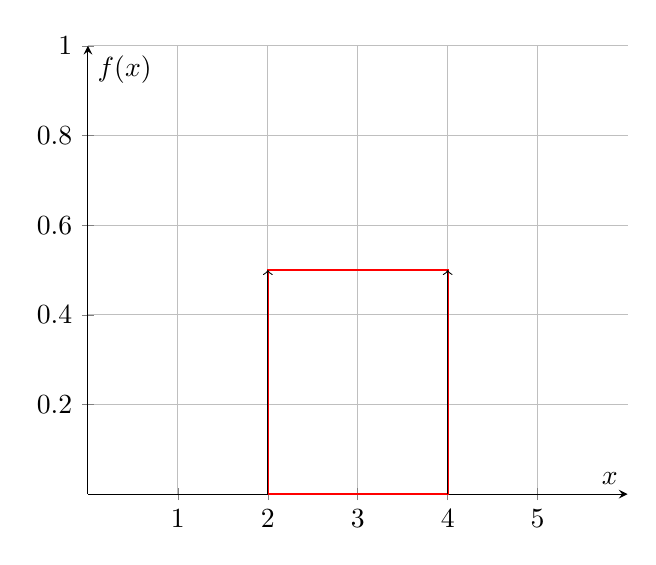
\begin{tikzpicture}
        \begin{axis}[
            axis lines = middle,
            xlabel = \( x \),
            ylabel = \( f(x) \),
            xmin = 0, xmax = 6,
            ymin = 0, ymax = 1,
            xtick={1,2,3,4,5},
            ytick={0.2,0.4,0.6,0.8,1.0},
            grid = both,
            domain=0:6,
            samples=50,
            legend pos=outer north east,
            ]
            \addplot[red, thick] coordinates {(2,0) (2,0.5) (4,0.5) (4,0) (2,0)};
            \draw[->] (2,0) -- (2,0.5);
            \draw[->] (4,0) -- (4,0.5);
            \node at (2,-0.1) {2};
            \node at (4,-0.1) {4};
        \end{axis}
    \end{tikzpicture}
    \end{center}

    The width of the rectangle (i.e., \( b - a \)) determines the range of possible values. A larger range decreases the height of the PDF, thus spreading the probability over a wider area. \\

    If \( X \) and \( Y \) are independent random variables each following a Uniform Distribution \( U(a, b) \), then the distribution of \( Z = X + Y \) can be determined. The sum of two independent Uniform random variables results in a triangular distribution over the interval \([2a, 2b]\). Specifically, the PDF of \( Z \) is piecewise linear, with its peak at \( a + b \).

\subsubsection{Exponential Distribution}

The Exponential Distribution is a continuous probability distribution that is widely used to model the time until an event occurs, such as the time until failure of a machine, the time between arrivals of customers in a queue, or the time until an earthquake. Its primary motivation lies in its memoryless property, which means that the future probability of an event occurring does not depend on how much time has already elapsed.\\

The Exponential Distribution is characterized by a single parameter, $\lambda > 0$, known as the rate parameter. 

\begin{definition}
    The PDF of the Exponential Distribution is defined as follows:
\[
f(x; \lambda) = 
\begin{cases} 
\lambda e^{-\lambda x} & \text{for } x \geq 0 \\
0 & \text{for } x < 0 
\end{cases}
\]
\end{definition}

\begin{proof}
    To derive this formula, we start from the definition of the cumulative distribution function (CDF):

\[
F(x; \lambda) = P(X \leq x) = 1 - e^{-\lambda x}, \quad x \geq 0
\]

Differentiating the CDF gives us the PDF:

\[
f(x; \lambda) = \frac{d}{dx}F(x; \lambda) = \lambda e^{-\lambda x}
\]

This derivation shows how the exponential decay characterizes the time until an event occurs.
\end{proof}

The shape of the Exponential Distribution is characterized by its PDF, which is a monotonically decreasing function. 
\begin{center}
    
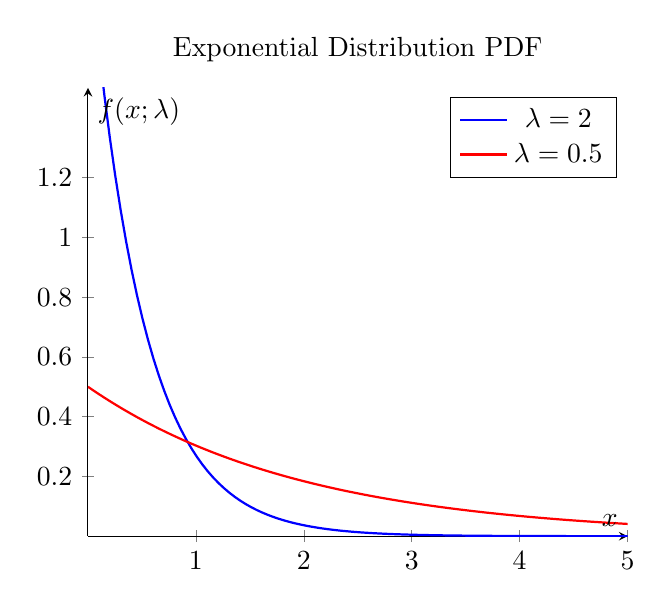
\begin{tikzpicture}
    \begin{axis}[
        axis lines=middle,
        xlabel={$x$},
        ylabel={$f(x; \lambda)$},
        title={Exponential Distribution PDF},
        ymin=0, ymax=1.5,
        xmin=0, xmax=5,
        xtick={0,1,2,3,4,5},
        ytick={0,0.2,0.4,0.6,0.8,1.0,1.2},
        domain=0:5,
        samples=100,
    ]
    \addplot[blue, thick] {2*exp(-2*x)}; % For λ = 2
    \addlegendentry{$\lambda = 2$}
    
    \addplot[red, thick] {0.5*exp(-0.5*x)}; % For λ = 0.5
    \addlegendentry{$\lambda = 0.5$}
    \end{axis}
    \end{tikzpicture}
\end{center}

The parameter $\lambda$ significantly impacts the shape of the distribution:
\begin{itemize}
    \item A larger $\lambda$ results in a steeper decline, meaning events occur more frequently (shorter waiting times).
    \item A smaller $\lambda$ leads to a slower decline, indicating longer waiting times between events.
\end{itemize}

For example, with $\lambda = 2$, the average time until the next event is $\frac{1}{2} = 0.5$ units of time, while with $\lambda = 0.5$, it is $\frac{1}{0.5} = 2$ units of time.\\

If $X$ and $Y$ are independent random variables that follow an Exponential Distribution with the same parameter $\lambda$, the distribution of the sum $Z = X + Y$ follows a Gamma Distribution with shape parameter $k = 2$ and scale parameter $\theta = \frac{1}{\lambda}$:

\[
Z \sim \text{Gamma}(k=2, \theta=\frac{1}{\lambda})
\]

The PDF of $Z$ is given by:

\[
f_Z(z; \lambda) = \frac{\lambda^2 z e^{-\lambda z}}{1!}, \quad z \geq 0
\]

We will look at the Gamma Distribution shortly. 

\begin{example}
    Consider a scenario where a factory produces light bulbs, and the average lifespan of a bulb is 1000 hours, which means $\lambda = \frac{1}{1000}$ hours$^{-1}$. \\

If we want to model the time until the next bulb fails, we use the Exponential Distribution. The probability that a bulb will last more than 1200 hours is calculated as follows:

\[
P(X > 1200) = 1 - P(X \leq 1200) = 1 - F(1200; \lambda) = e^{-\frac{1200}{1000}} \approx e^{-1.2} \approx 0.3012
\]

This means there is approximately a 30.12\% chance that the bulb will last longer than 1200 hours.

\end{example}

\subsubsection{Normal Distribution}

The Normal Distribution, also known as the Gaussian distribution, is fundamental in statistics and probability theory. It is crucial for modeling phenomena that tend to cluster around a mean. Many natural occurrences—like heights, test scores, and measurement errors—are often normally distributed. \\

The Normal Distribution is characterized by two parameters:
\begin{itemize}
    \item $\mu$: The mean, which indicates the center of the distribution.
    \item $\sigma$: The standard deviation, which measures the dispersion or spread of the distribution.
\end{itemize}
These parameters define the behavior of the distribution and its shape.

\begin{definition}
    The PDF of a Normal Distribution is given by:
\[
f(x) = \frac{1}{\sigma \sqrt{2\pi}} e^{-\frac{(x - \mu)^2}{2\sigma^2}}
\]
\end{definition}

\begin{proof}
    The PDF must satisfy two properties:
\begin{enumerate}
    \item It is non-negative: \(f(x) \geq 0\) for all \(x\).
    \item It integrates to one over the entire space:
    \[
    \int_{-\infty}^{\infty} f(x) \, dx = 1
    \]
\end{enumerate}

We want a function \(f(x)\) such that it is symmetric on both sides of its mean, allows straightforward integration, decays quickly after the mean - preferably exponentially. The function that fits these criteria is $f(x) = A e^{-B(x - \mu)^2}$. It's a bell-curve and a good choice because the shape produced by the exponential function is bell-like, which is a natural representation of many real-world phenomena that cluster around a central value. In various fields, such as physics and natural sciences, phenomena like diffusion and heat conduction can be modeled using exponential decay. This physical foundation supports the choice of the exponential function for representing distributions that describe natural processes.\\

To satisfy the normalization condition, we need:

\[
\int_{-\infty}^{\infty} A e^{-B(x - \mu)^2} \, dx = 1
\]

Changing variables to \(z = x - \mu\), we have:

\[
\int_{-\infty}^{\infty} A e^{-Bz^2} \, dz = 1
\]

This integral is known as the Gaussian integral:

\[
\int_{-\infty}^{\infty} e^{-Bz^2} \, dz = \sqrt{\frac{\pi}{B}}
\]

Thus, we have:

\[
A \sqrt{\frac{\pi}{B}} = 1 \implies A = \sqrt{\frac{B}{\pi}}
\]

Let \(B = \frac{1}{2\sigma^2}\):

\[
f(x) = \sqrt{\frac{1}{2\pi \sigma^2}} e^{-\frac{(x - \mu)^2}{2\sigma^2}}
\]

This satisfies the normalization condition. Finally, we express the PDF in its standard form:

\[
f(x) = \frac{1}{\sigma \sqrt{2\pi}} e^{-\frac{(x - \mu)^2}{2\sigma^2}}
\]
\end{proof}

\begin{definition}
    The standard normal curve is a special case of the normal distribution where the mean \(\mu\) is \(0\) and the standard deviation \(\sigma\) is \(1\). It is denoted as \(N(0, 1)\) and is symmetrical about the mean. The equation of the standard normal distribution is given by:

    \[
f(z) = \frac{1}{\sqrt{2\pi}} e^{-\frac{z^2}{2}}
\]

where \(z\) represents the z-score.
\end{definition}

\begin{definition}
    A z-score indicates how many standard deviations an element is from the mean of the distribution. It is calculated using the formula:

\[
z = \frac{(X - \mu)}{\sigma}
\]

where:
\begin{itemize}
    \item \(X\) is the value of the observation,
    \item \(\mu\) is the mean of the distribution,
    \item \(\sigma\) is the standard deviation.
\end{itemize}
\end{definition}

A positive z-score indicates that the value is above the mean, while a negative z-score indicates that it is below the mean. The z-score is crucial for standardizing values from different normal distributions to the standard normal distribution, allowing for comparison across different datasets.\\

The Normal Distribution is symmetric and bell-shaped. Its key characteristics include:
\begin{itemize}
    \item \textbf{Mean ($\mu$)}: The peak of the bell curve.
    \item \textbf{Standard Deviation ($\sigma$)}: Determines the width of the curve. A smaller $\sigma$ results in a steeper curve, while a larger $\sigma$ produces a flatter curve.
\end{itemize}

\begin{center}
    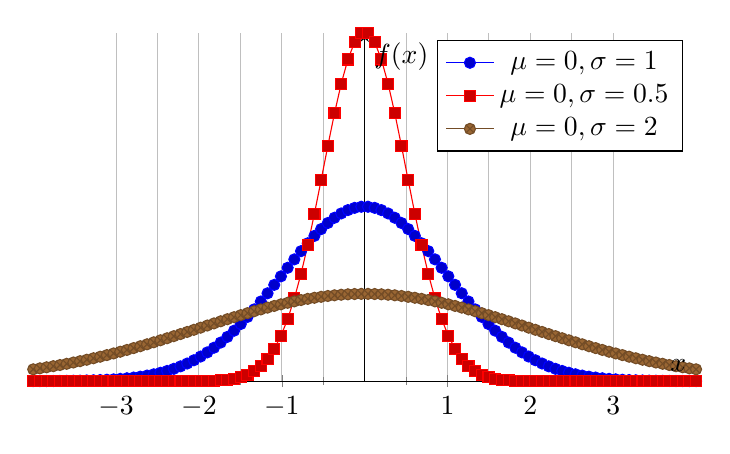
\begin{tikzpicture}
        \begin{axis}[
            axis lines = middle,
            xlabel = $x$,
            ylabel = {$f(x)$},
            xtick={-3,-2,-1,0,1,2,3},
            ytick=\empty,
            domain=-4:4,
            samples=100,
            width=10cm,
            height=6cm,
            grid=both,
            minor tick num=1,
            ]
            % Normal Distribution with mu = 0, sigma = 1
            \addplot {1/(sqrt(2*pi)*1) * exp(-((x-0)^2)/(2*1^2))};
            \addlegendentry{$\mu=0, \sigma=1$}
            
            % Normal Distribution with mu = 0, sigma = 0.5
            \addplot {1/(sqrt(2*pi)*0.5) * exp(-((x-0)^2)/(2*0.5^2))};
            \addlegendentry{$\mu=0, \sigma=0.5$}
            
            % Normal Distribution with mu = 0, sigma = 2
            \addplot {1/(sqrt(2*pi)*2) * exp(-((x-0)^2)/(2*2^2))};
            \addlegendentry{$\mu=0, \sigma=2$}
            
        \end{axis}
    \end{tikzpicture}
    \end{center}

The graph illustrates the effect of varying standard deviations on the distribution's shape. For example:
\begin{itemize}
    \item When $\sigma = 0.5$, the distribution is narrow and peaked.
    \item When $\sigma = 2$, the distribution is wider and flatter.
\end{itemize} 

If \(X\) and \(Y\) are independent random variables, both following a Normal Distribution:
\[
X \sim N(\mu_X, \sigma_X^2), \quad Y \sim N(\mu_Y, \sigma_Y^2)
\]
Then, the sum \(Z = X + Y\) is also normally distributed:
\[
Z \sim N(\mu_X + \mu_Y, \sigma_X^2 + \sigma_Y^2)
\]

\begin{example}
    Suppose the heights of adult men in a certain city are normally distributed with a mean of \(\mu = 175\) cm and a standard deviation of \(\sigma = 10\) cm. \\

Calculate the following:
\begin{enumerate}
    \item The z-score for a man who is 190 cm tall.
    \item The probability that a randomly selected man from this city is taller than 190 cm.
\end{enumerate}

The z-score is calculated using the formula:

\[
z = \frac{(X - \mu)}{\sigma}
\]

where:
\begin{itemize}
    \item \(X\) is the value for which we want to find the z-score,
    \item \(\mu\) is the mean,
    \item \(\sigma\) is the standard deviation.
\end{itemize}

For a man who is \(X = 190\) cm tall:

\[
z = \frac{(190 - 175)}{10} = \frac{15}{10} = 1.5
\]

To find the probability that a randomly selected man is taller than 190 cm, we look up the z-score in the standard normal distribution table or use a cumulative distribution function (CDF) calculator. \\

The CDF gives the probability that a random variable is less than a certain value. Thus, we need to find:

\[
P(X > 190) = 1 - P(X \leq 190) = 1 - P(Z \leq 1.5)
\]

From standard normal distribution tables, we find:

\[
P(Z \leq 1.5) \approx 0.9332
\]

Therefore, the probability is:

\[
P(X > 190) = 1 - 0.9332 = 0.0668
\]

The z-score for a man who is 190 cm tall is \(1.5\), and the probability that a randomly selected man from this city is taller than 190 cm is approximately \(0.0668\), or \(6.68\%\).

\end{example}

\subsubsection{Log-Normal Distribution}

The Log-Normal distribution is a continuous probability distribution of a random variable whose logarithm is normally distributed. It is commonly used to model variables that are multiplicative in nature, such as stock prices, income distributions, and the sizes of living organisms. \\

The primary parameters involved in modeling a Log-Normal distribution are:
\begin{itemize}
    \item $\mu$: the mean of the underlying normal distribution (i.e., the logarithm of the variable).
    \item $\sigma$: the standard deviation of the underlying normal distribution.
\end{itemize}

\begin{definition}
    The PDF of the Log-Normal distribution is defined as follows:
\[
f(x; \mu, \sigma) = \frac{1}{x \sigma \sqrt{2\pi}} e^{-\frac{(\ln x - \mu)^2}{2\sigma^2}}, \quad x > 0
\]
\end{definition}

\begin{proof}
    We start from the fact that if \( Y \) is normally distributed, i.e., \( Y \sim N(\mu, \sigma^2) \), then the random variable \( X = e^Y \) follows a Log-Normal distribution. The transformation of variables provides us with the PDF. Start with the PDF of normal distribution:

    \[
f_Y(y) = \frac{1}{\sigma \sqrt{2\pi}} e^{-\frac{(y - \mu)^2}{2\sigma^2}}
\]

Apply the transformation \( x = e^y \), which implies \( y = \ln x \) and \( dy = \frac{1}{x} dx \).\\

The PDF of \( X \) is then obtained using the change of variable:
\[
f_X(x) = f_Y(\ln x) \cdot \left| \frac{dy}{dx} \right| = f_Y(\ln x) \cdot \frac{1}{x}
\]

Substituting \( f_Y(\ln x) \) yields the PDF of the Log-Normal distribution as stated above.
\end{proof}

The shape of the Log-Normal distribution is positively skewed, meaning it has a long tail on the right side. The parameters $\mu$ and $\sigma$ significantly impact its shape:

\begin{itemize}
    \item As $\mu$ increases, the peak of the distribution shifts to the right, indicating a higher central tendency.
    \item An increase in $\sigma$ increases the spread of the distribution, resulting in a wider and flatter shape. Conversely, a smaller $\sigma$ leads to a steeper peak.
\end{itemize}

\begin{center}
    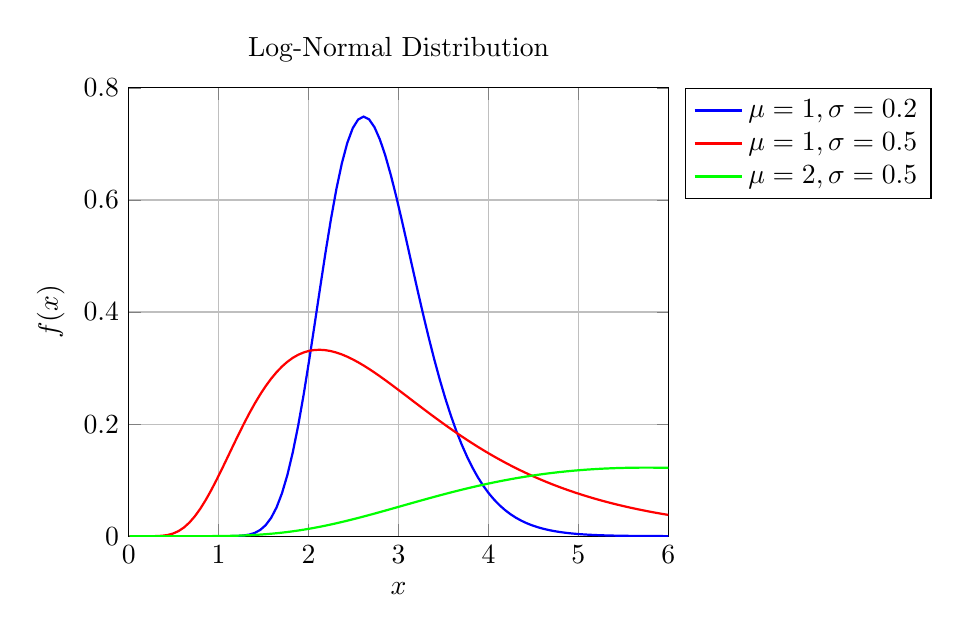
\begin{tikzpicture}
        \begin{axis}[
            title={Log-Normal Distribution},
            xlabel={$x$},
            ylabel={$f(x)$},
            xmin=0, xmax=6,
            ymin=0, ymax=0.8,
            legend pos=outer north east,
            grid=major,
            domain=0.01:6,
            samples=100
        ]
        \addplot[blue, thick] {1/(x*0.2*sqrt(2*pi))*exp(-((ln(x)-1)^2)/(2*0.2^2))}; 
        \addlegendentry{$\mu=1, \sigma=0.2$}
    
        \addplot[red, thick] {1/(x*0.5*sqrt(2*pi))*exp(-((ln(x)-1)^2)/(2*0.5^2))}; 
        \addlegendentry{$\mu=1, \sigma=0.5$}
    
        \addplot[green, thick] {1/(x*0.5*sqrt(2*pi))*exp(-((ln(x)-2)^2)/(2*0.5^2))}; 
        \addlegendentry{$\mu=2, \sigma=0.5$}
        \end{axis}
    \end{tikzpicture}
    \end{center}

    For example, with $\mu = 1$ and $\sigma = 0.2$, the distribution is relatively concentrated around the mean, while with $\sigma = 0.5$, it spreads out more, showing the impact of increasing variance.\\

    If \( X \) and \( Y \) are independent random variables that follow a Log-Normal distribution, specifically \( X \sim \text{Log-Normal}(\mu_X, \sigma_X^2) \) and \( Y \sim \text{Log-Normal}(\mu_Y, \sigma_Y^2) \), the distribution of the sum \( Z = X + Y \) does not follow a Log-Normal distribution. \\

However, there are approximations to understand the distribution of \( Z \). In some cases, the sum of two Log-Normal random variables can be approximated using a Normal distribution or simulated using numerical methods, depending on the parameters.

\begin{example}
    Consider the modeling of the future price of a stock that currently has a price of $P_0 = 100$. Assuming that the logarithm of the price follows a Normal distribution with parameters \( \mu = 0.05 \) and \( \sigma = 0.1 \):\\

1. We simulate the future price of the stock after 1 year:
\[
P = P_0 \cdot e^{Y}
\]
where \( Y \sim N(0.05, 0.1^2) \).\\

2. If we calculate the expected price and the variance, we can understand the distribution of future prices.\\

This modeling helps investors understand the risks and potential returns associated with stock investments, providing a probabilistic framework for decision-making.
\end{example}

\subsubsection{Weibull Distribution}

The Weibull distribution is a continuous probability distribution that is widely used in reliability analysis and failure time analysis. It is particularly useful in modeling life data, where it can describe the time until an event occurs, such as failure of a mechanical component or time to death in survival studies.\\

\begin{definition}
    The PDF of the Weibull distribution is given by:

\[
f(x; k, \lambda) = 
\begin{cases} 
\frac{k}{\lambda} \left( \frac{x}{\lambda} \right)^{k-1} e^{-(x/\lambda)^{k}} & \text{for } x \geq 0 \\
0 & \text{for } x < 0 
\end{cases}
\]
\end{definition}

\begin{proof}
    To derive this PDF, we start with the cumulative distribution function (CDF), defined as:

\[
F(x; k, \lambda) = 1 - e^{-(x/\lambda)^{k}} \quad \text{for } x \geq 0
\]

Taking the derivative of the CDF with respect to $x$ yields the PDF:

\[
f(x; k, \lambda) = \frac{d}{dx} F(x; k, \lambda) = \frac{d}{dx} \left( 1 - e^{-(x/\lambda)^{k}} \right) = \frac{k}{\lambda} \left( \frac{x}{\lambda} \right)^{k-1} e^{-(x/\lambda)^{k}}
\]
\end{proof}

The shape of the Weibull distribution is heavily influenced by the shape parameter $k$:

\begin{itemize}
    \item If $k < 1$: The distribution is decreasing; it indicates that the failure rate decreases over time (e.g., "infant mortality").
    \item If $k = 1$: The distribution is exponential, implying a constant failure rate.
    \item If $k > 1$: The distribution is increasing; it indicates that the failure rate increases over time (e.g., "wear-out failures").
\end{itemize}

The scale parameter $\lambda$ stretches or compresses the distribution along the x-axis. A larger $\lambda$ results in a distribution that spreads out more, while a smaller $\lambda$ makes it steeper.

\begin{center}
    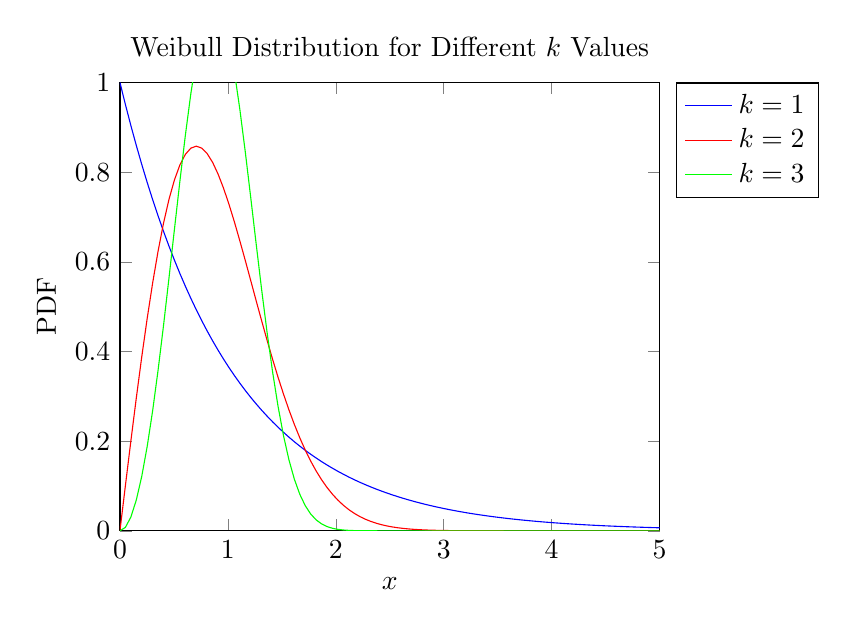
\begin{tikzpicture}
        \begin{axis}[
            xlabel={$x$},
            ylabel={PDF},
            xmin=0, xmax=5,
            ymin=0, ymax=1,
            title={Weibull Distribution for Different $k$ Values},
            legend pos=outer north east,
            samples=100
        ]
        \addplot[domain=0:5, color=blue]{(1/1) * (x/1)^(1-1) * exp(-(x/1)^1)};
        \addlegendentry{$k=1$}
        
        \addplot[domain=0:5, color=red]{(2/1) * (x/1)^(2-1) * exp(-(x/1)^2)};
        \addlegendentry{$k=2$}
        
        \addplot[domain=0:5, color=green]{(3/1) * (x/1)^(3-1) * exp(-(x/1)^3)};
        \addlegendentry{$k=3$}
        \end{axis}
    \end{tikzpicture}
    \end{center}

    In this graph, we see the differences in the shapes for $k=1$, $k=2$, and $k=3$.\\

    If $X$ and $Y$ are independent random variables following the Weibull distribution with the same scale parameter $\lambda$ and shape parameter $k$, the distribution of $X + Y$ is not generally a Weibull distribution. However, if both are identically distributed, we can use techniques such as convolution to find the PDF of $Z = X + Y$. The resulting distribution would require numerical methods for specific parameters and is generally not expressible in a closed form.

    \begin{example}
        Suppose the shape parameter is found to be $k=1.5$ and the scale parameter is $\lambda=1000$ hours. This indicates that the bulbs experience increasing failure rates as time progresses. The company can use this model to predict the reliability of their bulbs, estimating that approximately 63\% of the bulbs will have failed by 1000 hours.
    \end{example}

\subsubsection{Gamma Distribution}

The Gamma distribution is a continuous probability distribution that is widely used to model various processes, particularly those that involve waiting times or the time until an event occurs. Its flexibility makes it suitable for a variety of applications, including queuing models, reliability analysis, and Bayesian statistics.\\

The Gamma distribution is characterized by two parameters: 
\begin{itemize}
    \item \(\alpha\) (shape parameter): This parameter dictates the shape of the distribution. It is a positive real number that influences the skewness and the peak of the distribution.
    \item \(\beta\) (rate parameter): This parameter is also a positive real number, and it controls the scale of the distribution. It is often expressed as the reciprocal of the scale parameter \(\theta\) (where \(\theta = \frac{1}{\beta}\)).
\end{itemize}

Before diving into the Gamma distribution, it is essential to understand the Gamma function, which is defined as:
\[
\Gamma(n) = \int_0^\infty t^{n-1} e^{-t} \, dt
\]
for \( n > 0 \). The Gamma function generalizes the factorial function to real and complex numbers, with the relationship:
\[
\Gamma(n) = (n-1)!
\]
for natural numbers \( n \). The derivation of the Gamma function arises from the need to extend the concept of factorial to non-integer values, facilitating calculations in various mathematical fields, particularly in calculus and complex analysis.

\begin{definition}
    The PDF of the Gamma distribution is given by:
\[
f(x; \alpha, \beta) = \frac{\beta^\alpha}{\Gamma(\alpha)} x^{\alpha-1} e^{-\beta x}, \quad x > 0
\]
where \(\Gamma(\alpha)\) is the Gamma function.
\end{definition}

Before we dive into the proof of this PDF, we will need some results. 

\begin{theorem}
    The PDF of the sum of two independent random variables is the convolution of their PDFs. 
\end{theorem}

\begin{proof}
    Let \(Z = X + Y\). We want to find the PDF \(f_Z(z)\) of the random variable \(Z\).\\

    To derive \(f_Z(z)\), we can first find the cumulative distribution function (CDF) \(F_Z(z)\):
\[
F_Z(z) = P(Z \leq z) = P(X + Y \leq z).
\]

Given the independence of \(X\) and \(Y\), we can express the probability \(P(X + Y \leq z)\) as:
\[
F_Z(z) = \int_{-\infty}^{\infty} P(X \leq z - y) f_Y(y) \, dy.
\]

Here, \(P(X \leq z - y)\) is the CDF of \(X\), denoted by \(F_X(z - y)\):
\[
F_Z(z) = \int_{-\infty}^{\infty} F_X(z - y) f_Y(y) \, dy.
\]

To find the PDF \(f_Z(z)\), we differentiate \(F_Z(z)\) with respect to \(z\):
\[
f_Z(z) = \frac{d}{dz} F_Z(z) = \frac{d}{dz} \int_{-\infty}^{\infty} F_X(z - y) f_Y(y) \, dy.
\]

Using the Leibniz rule for differentiating under the integral sign, we have:
\[
f_Z(z) = \int_{-\infty}^{\infty} \frac{\partial}{\partial z} F_X(z - y) f_Y(y) \, dy.
\]

Since \(F_X(z - y)\) is the CDF of \(X\), its derivative is the PDF \(f_X(z - y)\):
\[
\frac{\partial}{\partial z} F_X(z - y) = f_X(z - y).
\]

Thus,
\[
f_Z(z) = \int_{-\infty}^{\infty} f_X(z - y) f_Y(y) \, dy.
\]

The expression we derived for \(f_Z(z)\) is the convolution of the PDFs \(f_X\) and \(f_Y\):
\[
f_Z(z) = (f_X * f_Y)(z) = \int_{-\infty}^{\infty} f_X(z - y) f_Y(y) \, dy.
\]

Therefore, we have shown that the PDF of the sum of two independent random variables \(Z = X + Y\) can be found using the convolution of their PDFs:
\[
f_Z(z) = f_X(z) * f_Y(z).
\]
\end{proof}

Now we can prove the PDF of the Gamma Distribution. The Gamma Distribution should be viewed as the Sum of Independent Exponential Random Variables. Let's prove this. 

\begin{proof}
    Let \(X_1, X_2, \ldots, X_k\) be \(k\) independent random variables, each following an exponential distribution with rate \(\beta\). The PDF of each \(X_i\) is given by:
\[
f_{X_i}(x) = \beta e^{-\beta x}, \quad x \geq 0.
\]

Define \(Y = X_1 + X_2 + \ldots + X_k\). We want to find the PDF of \(Y\).\\

The PDF of the sum of two independent random variables can be found using the convolution of their PDFs. The convolution of two PDFs \(f_X(x)\) and \(f_Y(y)\) is defined as:
\[
(f_X * f_Y)(z) = \int_0^z f_X(x) f_Y(z - x) \, dx.
\]

First, we find the PDF of \(Z = X_1 + X_2\):
\[
f_Z(z) = \int_0^z f_{X_1}(x) f_{X_2}(z - x) \, dx.
\]
Substituting the PDFs of the exponential distributions:
\[
f_Z(z) = \int_0^z \beta e^{-\beta x} \cdot \beta e^{-\beta (z - x)} \, dx.
\]
This simplifies to:
\[
f_Z(z) = \beta^2 e^{-\beta z} \int_0^z dx = \beta^2 e^{-\beta z} \cdot z.
\]
Thus,
\[
f_Z(z) = \beta^2 z e^{-\beta z}, \quad z \geq 0.
\]

Now, let's generalize this for \(k\) independent exponential random variables. We can derive it step by step:
1. Assume \(Y_k = X_1 + X_2 + \ldots + X_k\).
2. We already have the result for \(k=2\):
   \[
   f_{Y_2}(y) = \beta^2 y e^{-\beta y}.
   \]

Now, using the result for \(k=2\), we find the PDF of \(Y_k\) as follows:
\[
f_{Y_k}(y) = \int_0^y f_{Y_{k-1}}(x) f_{X_k}(y - x) \, dx.
\]
Substituting \(f_{Y_{k-1}}(x)\) and \(f_{X_k}(y - x)\):
\[
f_{Y_k}(y) = \int_0^y \left( \frac{\beta^{k-1}}{\Gamma(k-1)} x^{k-2} e^{-\beta x} \right) \left( \beta e^{-\beta (y - x)} \right) \, dx.
\]
This simplifies to:
\[
f_{Y_k}(y) = \beta^k e^{-\beta y} \int_0^y \frac{x^{k-2}}{\Gamma(k-1)} \, dx.
\]
The integral evaluates to:
\[
\int_0^y x^{k-2} \, dx = \frac{y^{k-1}}{k-1}.
\]
Thus, we have:
\[
f_{Y_k}(y) = \beta^k e^{-\beta y} \cdot \frac{y^{k-1}}{\Gamma(k)}.
\]
Thus, the PDF of \(Y = X_1 + X_2 + \ldots + X_k\) is given by:
\[
f_Y(y) = \frac{\beta^k}{\Gamma(k)} y^{k-1} e^{-\beta y}, \quad y \geq 0.
\]

This is the PDF of the Gamma distribution with shape parameter \(k\) and rate parameter \(\beta\). Therefore, we have proven that the Gamma distribution can be viewed as the sum of \(k\) independent exponentially distributed random variables.
\end{proof}

The shape of the Gamma distribution is highly influenced by its parameters \(\alpha\) and \(\beta\). 

\begin{itemize}
    \item For \(\alpha = 1\): The Gamma distribution simplifies to an exponential distribution, characterized by a single peak.
    \item For \(\alpha > 1\): The distribution becomes increasingly bell-shaped, with the peak shifting to the right as \(\alpha\) increases.
    \item For \(\alpha < 1\): The distribution is skewed to the right, approaching zero as \(x\) increases.
\end{itemize}

\begin{center}
    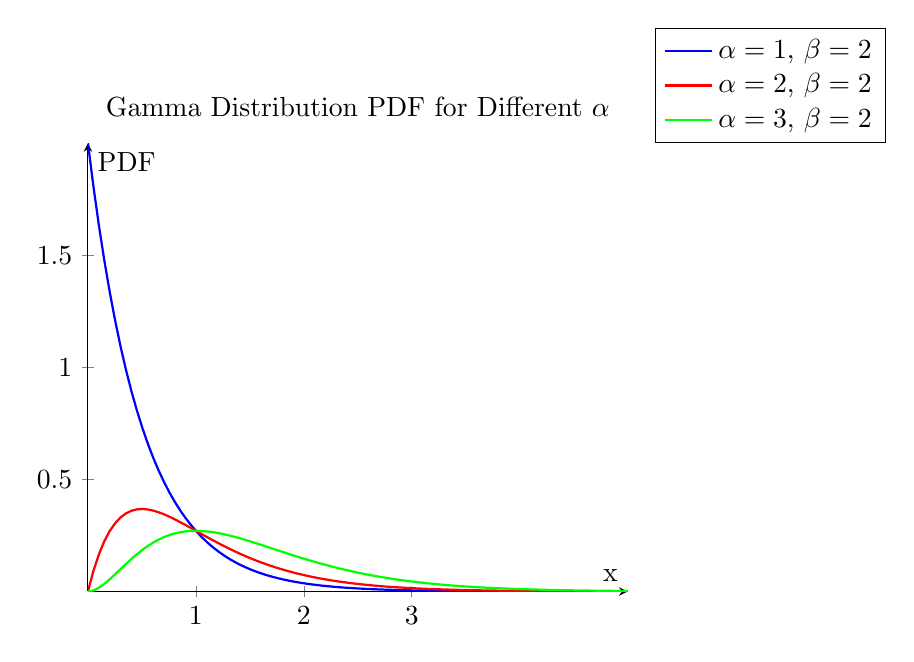
\begin{tikzpicture}
        \begin{axis}[
            axis lines = middle,
            xlabel = {x},
            ylabel = {PDF},
            xtick={0,1,2,3},
            ytick={0,0.5,1,1.5},
            domain=0:5,
            samples=100,
            legend style={at={(1.05,1)},anchor=south west},
            title={Gamma Distribution PDF for Different $\alpha$}
        ]
        \addplot[blue, thick] {2*exp(-2*x)}; % alpha = 1
        \addlegendentry{$\alpha = 1$, $\beta = 2$}
        
        \addplot[red, thick] {0.5*2^2*x*exp(-2*x)}; % alpha = 2
        \addlegendentry{$\alpha = 2$, $\beta = 2$}
        
        \addplot[green, thick] {0.5*2^3*x^2*exp(-2*x)/2}; % alpha = 3
        \addlegendentry{$\alpha = 3$, $\beta = 2$}
        \end{axis}
    \end{tikzpicture}
    \end{center}

    If \(X\) and \(Y\) are independent random variables each following a Gamma distribution with parameters \((\alpha_1, \beta)\) and \((\alpha_2, \beta)\) respectively, then the distribution of \(X + Y\) is given by:
    \[
    X + Y \sim \Gamma(\alpha_1 + \alpha_2, \beta)
    \]
    This property is significant in various applications, such as queuing theory, where the total waiting time can be modeled using the sum of Gamma-distributed random variables.

    \begin{example}
        Suppose a call center receives calls according to a Poisson process with an average rate of \(\lambda = 5\) calls per hour. The waiting time until the \(k\)-th call can be modeled using a Gamma distribution. \\

If we want to find the distribution of the waiting time for the 3rd call (\(X \sim \Gamma(3, \lambda)\)), we can determine the expected waiting time as:
\[
E[X] = \frac{\alpha}{\beta} = \frac{3}{5} = 0.6 \text{ hours} \quad (\text{or } 36 \text{ minutes})
\]
In this scenario, the Gamma distribution helps assess service times and manage resource allocation effectively.
    \end{example}

\subsubsection{Beta Distribution}

The Beta distribution is a continuous probability distribution defined on the interval \([0, 1]\). It is particularly useful in modeling random variables that represent proportions or probabilities. The motivation behind the Beta distribution arises from the need to model outcomes that are constrained within a finite range. The Beta distribution has widespread applications, particularly in Bayesian statistics, project management (e.g., PERT charts), and quality control. For instance, in project management, the Beta distribution can model the completion time of a project where the completion time is uncertain. \\

The Beta distribution is characterized by two shape parameters, \(\alpha\) and \(\beta\), which control the distribution's shape. The parameters represent the number of successes and failures, respectively, in a binomial distribution. Before delving into the Beta distribution, it's essential to understand the Beta function, which serves as the normalization constant for the Beta distribution. \\

The Beta function, denoted as \(B(x, y)\), is defined as:

\[
B(x, y) = \int_0^1 t^{x-1} (1 - t)^{y-1} dt
\]

This integral arises in various areas of mathematics, particularly in calculus and combinatorial analysis. The Beta function can be related to the Gamma function via the identity:

\[
B(x, y) = \frac{\Gamma(x) \Gamma(y)}{\Gamma(x + y)}
\]

The Beta function is used to normalize the Beta distribution, ensuring that the total area under the probability density function (PDF) equals 1.

\begin{definition}
    The PDF of the Beta distribution is given by:

\[
f(x; \alpha, \beta) = \frac{x^{\alpha - 1} (1 - x)^{\beta - 1}}{B(\alpha, \beta)} \quad \text{for } 0 < x < 1
\]

where \(\alpha > 0\) and \(\beta > 0\).
\end{definition}

\begin{proof}
    The PDF of the Beta distribution, denoted as \(f(x; \alpha, \beta)\), can be expressed as a function that needs to be normalized. We propose a form:

\[
f(x; \alpha, \beta) = C \cdot x^{\alpha - 1} (1 - x)^{\beta - 1}
\]

where \(C\) is a normalization constant.\\

To ensure that the PDF integrates to 1 over the interval \([0, 1]\), we must have:

\[
\int_0^1 f(x; \alpha, \beta) \, dx = 1
\]

Substituting our proposed form into this equation gives:

\[
\int_0^1 C \cdot x^{\alpha - 1} (1 - x)^{\beta - 1} \, dx = 1
\]

We recognize the left-hand side as the definition of the Beta function:

\[
C \cdot B(\alpha, \beta) = 1
\]

Thus, we find the normalization constant \(C\):

\[
C = \frac{1}{B(\alpha, \beta)}
\]

Substituting \(C\) back into our proposed PDF gives:

\[
f(x; \alpha, \beta) = \frac{1}{B(\alpha, \beta)} \cdot x^{\alpha - 1} (1 - x)^{\beta - 1}
\]
\end{proof}

The shape of the Beta distribution can vary significantly depending on the parameters \(\alpha\) and \(\beta\):

\begin{itemize}
    \item If \(\alpha = 1\) and \(\beta = 1\), the distribution is uniform on \([0, 1]\).
    \item If \(\alpha > 1\) and \(\beta = 1\), the distribution is increasing.
    \item If \(\alpha = 1\) and \(\beta > 1\), the distribution is decreasing.
    \item If \(\alpha > 1\) and \(\beta > 1\), the distribution is bell-shaped, peaking around \(\frac{\alpha - 1}{\alpha + \beta - 2}\).
    \item If \(\alpha < 1\) and \(\beta < 1\), the distribution has U-shape.
\end{itemize}

\begin{center}
    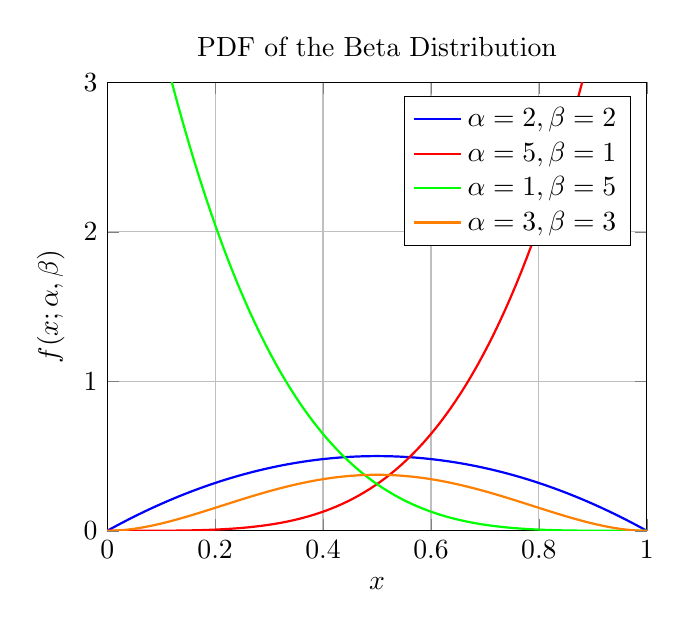
\begin{tikzpicture}
        \begin{axis}[
            xlabel={$x$},
            ylabel={$f(x; \alpha, \beta)$},
            xmin=0, xmax=1,
            ymin=0, ymax=3,
            domain=0:1,
            samples=100,
            legend pos=north east,
            grid=major,
            title={PDF of the Beta Distribution}
        ]
            % Plot for alpha = 2, beta = 2
            \addplot[blue, thick] {2 * x * (1 - x)};
            \addlegendentry{$\alpha = 2, \beta = 2$}
            
            % Plot for alpha = 5, beta = 1
            \addplot[red, thick] {5 * x^4};
            \addlegendentry{$\alpha = 5, \beta = 1$}
            
            % Plot for alpha = 1, beta = 5
            \addplot[green, thick] {5 * (1 - x)^4};
            \addlegendentry{$\alpha = 1, \beta = 5$}
            
            % Plot for alpha = 3, beta = 3
            \addplot[orange, thick] {6 * x^2 * (1 - x)^2};
            \addlegendentry{$\alpha = 3, \beta = 3$}
        \end{axis}
    \end{tikzpicture}
\end{center}

For example, when \(\alpha = 2\) and \(\beta = 2\), the distribution is symmetric around \(0.5\), while \(\alpha = 0.5\) and \(\beta = 0.5\) create a U-shaped distribution.\\

If \(X\) and \(Y\) are independent random variables that follow a Beta distribution, specifically \(X \sim \text{Beta}(\alpha_1, \beta_1)\) and \(Y \sim \text{Beta}(\alpha_2, \beta_2)\), the distribution of \(X + Y\) does not follow a standard distribution. However, under specific conditions (e.g., when both variables are scaled), the result can be approximated or analyzed using convolution techniques.\\

In general, the sum of two Beta variables requires numerical methods or simulations for precise analysis.

\begin{example}
    Suppose we have a project that requires three estimates: optimistic time (5 days), pessimistic time (15 days), and most likely time (10 days). We can use the Beta distribution to model the likelihood of completing the project within a certain timeframe. \\

    Let \(\alpha\) and \(\beta\) be determined based on these estimates using the formula:

\[
\alpha = \frac{(m - a)(b - m)}{(b - a)^2}, \quad \beta = \frac{(b - m)(m - a)}{(b - a)^2}
\]

where \(m\) is the most likely time, \(a\) is the optimistic time, and \(b\) is the pessimistic time.\\

In this case, the application of the Beta distribution helps project managers evaluate risk and optimize project timelines based on uncertainty.
\end{example}

\subsubsection{Chi-squared Distribution}
The Chi-squared distribution is a continuous probability distribution that arises in statistical inference, particularly in hypothesis testing and confidence interval estimation for population variance. It is commonly used to model the distribution of the sum of the squares of $k$ independent standard normal random variables. \\

To understand the motivation behind the Chi-squared distribution, consider that many statistical tests rely on estimating variances from sample data. When you collect data and calculate how far each data point is from the mean, you are effectively measuring variability. The Chi-squared distribution helps us determine whether the observed variability in our sample data is consistent with a certain population variance or if it indicates something unusual.\\

The parameters involved in this modeling include:
\begin{itemize}
    \item The number of degrees of freedom ($k$), which corresponds to the number of independent standard normal variables being squared and summed.
\end{itemize}

\begin{definition}
    The PDF of the Chi-squared distribution with $k$ degrees of freedom is given by:
\[
f(x; k) = \frac{1}{2^{k/2} \Gamma(k/2)} x^{(k/2)-1} e^{-x/2}, \quad \text{for } x > 0
\]
where $\Gamma$ is the Gamma function.
\end{definition}

\begin{proof}
    The Chi-squared distribution is defined as the distribution of the sum of the squares of $k$ independent standard normal random variables. This derivation will illustrate how we arrive at the probability density function (PDF) of the Chi-squared distribution.\\

    Let $Z \sim N(0, 1)$ be a standard normal random variable, which has the following PDF:
\[
f_Z(z) = \frac{1}{\sqrt{2\pi}} e^{-\frac{z^2}{2}}, \quad \text{for } -\infty < z < \infty.
\]

Consider $k$ independent standard normal random variables:
\[
Z_1, Z_2, \ldots, Z_k \sim N(0, 1.
\]
The Chi-squared variable is defined as:
\[
Y = Z_1^2 + Z_2^2 + \ldots + Z_k^2.
\]

To find the PDF of $Y$, we start with the joint distribution of the $Z_i$. The joint PDF of $Z_1, Z_2, \ldots, Z_k$ is given by:
\[
f_{Z_1, Z_2, \ldots, Z_k}(z_1, z_2, \ldots, z_k) = \prod_{i=1}^{k} f_Z(z_i) = \left(\frac{1}{\sqrt{2\pi}}\right)^k e^{-\frac{1}{2} \sum_{i=1}^{k} z_i^2}.
\]

Next, we make a change of variables from $Z_1, Z_2, \ldots, Z_k$ to $Y$ and the angles in polar coordinates, where:
\[
Y = Z_1^2 + Z_2^2 + \ldots + Z_k^2
\]
and the Jacobian determinant of the transformation will involve the angles.

The relationship in polar coordinates leads to:
\[
z_1^2 + z_2^2 + \ldots + z_k^2 = r^2
\]
where $r^2 = Y$. The angle terms introduce a factor of $\frac{(2\pi)^{k/2}}{(r^{k-1})}$ due to the transformation to polar coordinates.
We can then express the PDF of $Y$ as follows:
\[
f_Y(y) = \int_{\mathbb{R}^{k-1}} f_{Z_1, Z_2, \ldots, Z_k}(z_1, z_2, \ldots, z_k) \, dz_1 dz_2 \ldots dz_{k-1}.
\]
Substituting the expression for $f_{Z_1, Z_2, \ldots, Z_k}$ and integrating out the angular parts gives:
\[
f_Y(y) = \frac{1}{(2\pi)^{k/2}} \int_{0}^{2\pi} e^{-\frac{y}{2}} y^{(k/2)-1} \frac{(2\pi)^{k/2}}{(r^{k-1})} dr.
\]

After performing the integration, we arrive at:
\[
f_Y(y) = \frac{1}{2^{k/2} \Gamma(k/2)} y^{(k/2)-1} e^{-y/2}, \quad y > 0.
\]We can then express the PDF of $Y$ as follows:
\[
f_Y(y) = \int_{\mathbb{R}^{k-1}} f_{Z_1, Z_2, \ldots, Z_k}(z_1, z_2, \ldots, z_k) \, dz_1 dz_2 \ldots dz_{k-1}.
\]
Substituting the expression for $f_{Z_1, Z_2, \ldots, Z_k}$ and integrating out the angular parts gives:
\[
f_Y(y) = \frac{1}{(2\pi)^{k/2}} \int_{0}^{2\pi} e^{-\frac{y}{2}} y^{(k/2)-1} \frac{(2\pi)^{k/2}}{(r^{k-1})} dr.
\]

After performing the integration, we arrive at:
\[
f_Y(y) = \frac{1}{2^{k/2} \Gamma(k/2)} y^{(k/2)-1} e^{-y/2}, \quad y > 0.
\]Thus, we have derived the PDF of the Chi-squared distribution with $k$ degrees of freedom:
\[
f_Y(y) = \frac{1}{2^{k/2} \Gamma(k/2)} y^{(k/2)-1} e^{-y/2}, \quad y > 0.
\]
\end{proof}

The shape of the Chi-squared distribution depends significantly on the degrees of freedom ($k$):
\begin{itemize}
    \item For $k = 1$: The distribution is highly skewed to the right.
    \item For $k = 2$: The distribution starts to take on a more pronounced bell shape.
    \item As $k$ increases, the distribution becomes more symmetric and approaches a normal distribution \textit{(due to central limit theorem - will be studied later)}.
\end{itemize}

\begin{center}
    \begin{tikzpicture}
        \begin{axis}[
            title={Chi-squared Distribution},
            xlabel={$y$},
            ylabel={PDF},
            legend pos=outer north east,
            grid=major,
            domain=0:15,
            samples=100,
            ymin=0, ymax=0.4,
            unbounded coords=jump
        ]
        \addplot[blue, thick] {1/(2^(1/2)*tgamma(1/2))*x^(1/2-1)*exp(-x/2)};
        \addplot[red, thick] {1/(2^(2/2)*tgamma(2/2))*x^(2/2-1)*exp(-x/2)};
        \addplot[green, thick] {1/(2^(5/2)*tgamma(5/2))*x^(5/2-1)*exp(-x/2)};
        \legend{$k=1$, $k=2$, $k=5$}
        \end{axis}
    \end{tikzpicture}
    \end{center}

    
    For example:
    \begin{itemize}
        \item For $k = 1$, the peak is at $x = 0$, and it falls off steeply.
        \item For $k = 5$, the distribution is more spread out and has a more pronounced peak, making it resemble a normal distribution.
    \end{itemize}

    If $X \sim \chi^2(k_1)$ and $Y \sim \chi^2(k_2)$ are independent Chi-squared random variables, then the sum $Z = X + Y$ follows a Chi-squared distribution with $k_1 + k_2$ degrees of freedom:
\[
Z \sim \chi^2(k_1 + k_2)
\]

\begin{example}
    Consider a researcher testing whether a six-sided die is fair. They roll the die 60 times and record the frequency of each outcome. If the observed frequencies are significantly different from the expected frequencies (10 for each side), the researcher can use the Chi-squared test to determine whether the die is biased. The test statistic is calculated as:
\[
\chi^2 = \sum \frac{(O_i - E_i)^2}{E_i}
\]
where \(O_i\) is the observed frequency and \(E_i\) is the expected frequency. By comparing this statistic to the Chi-squared distribution with appropriate degrees of freedom, the researcher can draw conclusions about the fairness of the die.
\end{example}

\subsubsection{Student's t-Distribution}

When we collect data from a population, we often want to estimate the mean and understand the variability of that mean. However, if our sample size is small (typically less than 30), the sampling distribution of the sample mean follows a t-distribution rather than a normal distribution. \\

The parameters involved in this modeling include:
\begin{itemize}
    \item The sample size \( n \)
    \item The sample mean \( \bar{x} \)
    \item The sample standard deviation \( s \)
\end{itemize}

\begin{definition}
    The PDF of the Student's t-distribution is defined as:

\[
f(t) = \frac{\Gamma\left(\frac{v+1}{2}\right)}{\sqrt{v \pi} \, \Gamma\left(\frac{v}{2}\right)} \left(1 + \frac{t^2}{v}\right)^{-\frac{v+1}{2}}
\]

where \( v \) is the degrees of freedom and \( \Gamma \) is the gamma function.
\end{definition}

\begin{proof}
    The Student's t-distribution arises when we estimate the mean of a normally distributed population with an unknown standard deviation. To derive its probability density function (PDF), we start with the following components.\\

    Given a sample of \( n \) observations \( X_1, X_2, \ldots, X_n \), the sample mean \( \bar{X} \) and sample standard deviation \( S \) are defined as:

   \[
   \bar{X} = \frac{1}{n} \sum_{i=1}^{n} X_i,
   \]
   \[
   S = \sqrt{\frac{1}{n-1} \sum_{i=1}^{n} (X_i - \bar{X})^2}.
   \]

   The t-statistic is defined as:

   \[
   t = \frac{\bar{X} - \mu}{S / \sqrt{n}},
   \]

   where \( \mu \) is the true population mean. \\

   If the underlying population is normally distributed, the numerator \( \bar{X} - \mu \) follows a normal distribution with mean \( 0 \) and variance \( \frac{\sigma^2}{n} \), where \( \sigma^2 \) is the population variance. The denominator \( S \) is independent of \( \bar{X} \) and follows a scaled chi-squared distribution. \\

   Assuming \( X_i \) follows a normal distribution \( \mathcal{N}(\mu, \sigma^2) \):

\[
\bar{X} \sim \mathcal{N}\left(\mu, \frac{\sigma^2}{n}\right).
\]

The sample variance \( S^2 \) follows a chi-squared distribution:

\[
\frac{(n-1)S^2}{\sigma^2} \sim \chi^2_{n-1}.
\]

The joint distribution of \( \bar{X} \) and \( S^2 \) can be expressed using their independence:

\[
f_{\bar{X}, S^2}(x, s^2) = f_{\bar{X}}(x) f_{S^2}(s^2).
\]

We need to express the distribution in terms of the t-statistic \( t \). By substituting \( t \) in terms of \( \bar{X} \) and \( S \):

\[
t = \frac{\sqrt{n}(\bar{X} - \mu)}{S}.
\]

To derive the PDF of \( t \), we must consider the transformation of variables and compute the Jacobian. The Jacobian of the transformation from \( (X, S) \) to \( (t, S) \) is given by:

\[
J = \frac{\partial(t, S)}{\partial(\bar{X}, S)} = \frac{\sqrt{n}}{S}.
\]

The PDF of the t-distribution can be derived using the joint distribution and the transformation:\\

1. The PDF of \( \bar{X} \) is given by:

   \[
   f_{\bar{X}}(x) = \frac{1}{\sqrt{2\pi \sigma^2/n}} \exp\left(-\frac{n(x - \mu)^2}{2\sigma^2}\right).
   \]

2. The PDF of \( S^2 \) follows a chi-squared distribution:

   \[
   f_{S^2}(s^2) = \frac{(n-1)^{(n-1)/2}}{\Gamma\left(\frac{n-1}{2}\right) \sqrt{2\pi s^2}} \left( \frac{s^2}{\sigma^2} \right)^{(n-3)/2} \exp\left(-\frac{(n-1)s^2}{2\sigma^2}\right).
   \]

3. Combining these and accounting for the Jacobian, we arrive at the PDF of the Student's t-distribution:

\[
f(t) = \frac{\Gamma\left(\frac{n}{2}\right)}{\sqrt{n \pi} \Gamma\left(\frac{n-1}{2}\right)} \left(1 + \frac{t^2}{n-1}\right)^{-\frac{n}{2}}.
\]

Thus, the PDF of the Student's t-distribution with \( n-1 \) degrees of freedom is given by:

\[
f(t) = \frac{\Gamma\left(\frac{v+1}{2}\right)}{\sqrt{v \pi} \, \Gamma\left(\frac{v}{2}\right)} \left(1 + \frac{t^2}{v}\right)^{-\frac{v+1}{2}},
\]

where \( v = n - 1 \) is the degrees of freedom.
\end{proof}

The shape of the Student's t-distribution is similar to the normal distribution but has heavier tails. This characteristic allows it to better account for the variability in estimates when sample sizes are small. 

\begin{center}
    
\begin{tikzpicture}
    \begin{axis}[
        axis lines = middle,
        xlabel = {$t$},
        ylabel = {$f(t)$},
        ymin = 0,
        domain = -4:4,
        samples = 100,
        xtick={-4,-3,-2,-1,0,1,2,3,4},
        ytick={0,0.1,0.2,0.3},
        legend pos=outer north east,
        title={Student's t-distribution with different degrees of freedom}
    ]
    \addplot[blue, thick] { (tgamma(3/2)/sqrt(1*pi*2) * (1+x^2/2)^(-3/2)) };
    \addlegendentry{$v = 1$}
    
    \addplot[red, thick] { (tgamma(4/2)/sqrt(2*pi) * (1+x^2/2)^(-4/2)) };
    \addlegendentry{$v = 2$}
    
    \addplot[green, thick] { (tgamma(5/2)/sqrt(3*pi) * (1+x^2/3)^(-5/2)) };
    \addlegendentry{$v = 3$}
    
    \addplot[orange, thick] { (tgamma(6/2)/sqrt(4*pi) * (1+x^2/4)^(-6/2)) };
    \addlegendentry{$v = 4$}
    
    \end{axis}
\end{tikzpicture}
\end{center}

The parameter \( v \) (degrees of freedom) greatly affects the distribution's shape:
\begin{itemize}
    \item As \( v \) increases, the distribution approaches the normal distribution.
    \item Smaller values of \( v \) lead to heavier tails, indicating a higher likelihood of extreme values.
\end{itemize}

For example, with \( v = 1 \), the distribution has very heavy tails, while with \( v = 30 \), it closely resembles the standard normal distribution.\\

If \( X \) and \( Y \) are independent random variables following a Student's t-distribution with \( v \) degrees of freedom, then the distribution of \( Z = X + Y \) is not straightforward. Generally, the sum of two independent t-distributed variables does not follow a t-distribution unless specific conditions are met. However, if both have the same degrees of freedom, their sum can be approximated by a normal distribution for large \( v \).

\begin{example}
    A common application of the Student's t-distribution is in the context of the two-sample t-test, which is used to determine whether two population means are significantly different from each other. \\

For example, suppose a researcher wants to compare the average heights of students in two different classes:\\

1. Collect heights from Class A (sample size \( n_A \)) and Class B (sample size \( n_B \)).\\
2. Calculate the sample means \( \bar{x}_A \) and \( \bar{x}_B \), and the standard deviations \( s_A \) and \( s_B \).\\
3. Use the two-sample t-test to evaluate the hypothesis that \( \mu_A = \mu_B \):

\[
t = \frac{\bar{x}_A - \bar{x}_B}{\sqrt{\frac{s_A^2}{n_A} + \frac{s_B^2}{n_B}}}
\]

4. Compare the calculated t-value with the critical t-value from the t-distribution table with \( v = n_A + n_B - 2 \) degrees of freedom.\\

If the calculated t-value exceeds the critical t-value, the null hypothesis is rejected, indicating a significant difference in the average heights of the two classes.

\end{example}

\section{Moments}

Let \( X \) be a random variable. 

\begin{definition}
    \begin{itemize}
        \item The mean, also called the \textit{expected value}, is the average value of the random variable. It is defined as:
        \[
        \mu = \mathbb{E}[X] = \int_{-\infty}^{\infty} x f_X(x) \, dx
        \]
        where \( f_X(x) \) is the probability density function (pdf) of \( X \) in the continuous case, or
        \[
        \mu = \mathbb{E}[X] = \sum_{x \in \text{Range}(X)} x P(X = x)
        \]
        in the discrete case.
        \item  The median is the value that separates the higher half from the lower half of the distribution. Formally, the median \( m \) satisfies:
        \[
        P(X \leq m) = 0.5
        \]
        In other words, 50\% of the probability mass is below the median. 
        \item The mode is the value of \( X \) that occurs with the highest frequency, or the value at which the probability density (or mass) function achieves its maximum:
        \[
        \text{Mode} = \arg \max_x f_X(x)
        \]
        where \( f_X(x) \) is the pdf in the continuous case or the probability mass function (pmf) in the discrete case.
    \end{itemize}
\end{definition}

\begin{definition}
    Let \( X \) be a random variable with mean \( \mu = E(X) \). The \textit{variance} of \( X \), denoted as \( \text{Var}(X) \) or \( \sigma^2 \), is defined as:

\[
\text{Var}(X) = E\left[(X - \mu)^2\right] = E(X^2) - \left(E(X)\right)^2.
\]
\end{definition}

Variance measures the expected squared deviation of \( X \) from its mean \( \mu \).

\begin{theorem}
    Let \( X \) be a random variable with mean \( \mu \), and let \( m \) be a median of \( X \).
\begin{itemize}
    \item The value of \( c \) that minimizes the mean squared error \( E[(X - c)^2] \) is \( c = \mu \).
    \item A value of \( c \) that minimizes the mean absolute error \( E[|X - c|] \) is \( c = m \).
\end{itemize}
\end{theorem}

\begin{proof}
    
\textbf{(i) Minimizing the Mean Squared Error:}\\

We want to minimize the mean squared error function:
\[
E[(X - c)^2] = \int_{-\infty}^{\infty} (x - c)^2 f_X(x) dx,
\]
where \( f_X(x) \) is the probability density function of \( X \). Expanding the square, we have:
\[
E[(X - c)^2] = \int_{-\infty}^{\infty} \left( (x - \mu)^2 + 2(x - \mu)(\mu - c) + (\mu - c)^2 \right) f_X(x) dx.
\]
Taking the derivative with respect to \( c \) and setting it to zero to find the minimizing value of \( c \):
\[
\frac{d}{dc} E[(X - c)^2] = -2 E[X - c] = -2 (\mu - c).
\]
Setting this equal to zero, we obtain \( c = \mu \). Therefore, the value of \( c \) that minimizes \( E[(X - c)^2] \) is the mean \( \mu \).\\

\textbf{(ii) Minimizing the Mean Absolute Error:}\\

Next, we want to minimize the mean absolute error function:
\[
E[|X - c|] = \int_{-\infty}^{\infty} |x - c| f_X(x) dx.
\]
To minimize this, we take the derivative of \( E[|X - c|] \) with respect to \( c \) and analyze the behavior of the function. The derivative is given by:
\[
\frac{d}{dc} E[|X - c|] = \int_{-\infty}^{\infty} \text{sign}(x - c) f_X(x) dx,
\]
where \( \text{sign}(x - c) \) is \( -1 \) for \( x < c \) and \( 1 \) for \( x > c \).

For the derivative to be zero, we require that the proportion of values of \( X \) less than \( c \) equals the proportion of values greater than \( c \), i.e.,
\[
P(X \leq c) = P(X \geq c) = \frac{1}{2}.
\]
Thus, \( c \) must be a median of the distribution of \( X \). Therefore, the value of \( c \) that minimizes \( E[|X - c|] \) is a median \( m \) of \( X \).
\end{proof}

\subsection{Interpreting Moments}

\begin{definition}
    Let \( X \) be a random variable with mean \( \mu \) and variance \( \sigma^2 \). For any positive integer \( n \), we define the following:

\begin{itemize}
    \item The \textit{nth moment} of \( X \) is \( E(X^n) \).
    \item The \textit{nth central moment} of \( X \) is \( E((X - \mu)^n) \).
    \item The \textit{nth standardized moment} of \( X \) is \( E\left( \left( \frac{X - \mu}{\sigma} \right)^n \right) \).
\end{itemize}

In the previous sentence, "if it exists" is left implicit.
\end{definition}

In probability and statistics, the term \textit{moment} is borrowed from physics, where moments describe the distribution of mass at a distance from a reference point. For a random variable (r.v.) \( X \) with mean \( \mu \) and variance \( \sigma^2 \), moments offer insight into the characteristics of the distribution of \( X \). In particular, the mean is the first moment, and the variance is the second central moment.\\

Let \( X \) be a discrete random variable with distinct possible values \( x_1, x_2, \dots, x_n \), and imagine a system where pebbles with masses \( m_j = P(X = x_j) \) are placed at each \( x_j \) on a number line. In this analogy, the mean \( E(X) \) corresponds to the \textit{center of mass} of the system, and the variance \( \text{Var}(X) \) corresponds to the \textit{moment of inertia} about the center of mass.\\

In physics, the center of mass is given by:
\[
E(X) = \sum_{j=1}^{n} m_j x_j,
\]
while the moment of inertia about the center of mass is:
\[
\text{Var}(X) = \sum_{j=1}^{n} m_j (x_j - E(X))^2.
\]
Thus, the mean (first moment) of a random variable corresponds to the center of mass of a system of pebbles, and the variance (second central moment) corresponds to the moment of inertia about this center of mass.\\

We now introduce the concept of skewness, which provides a single-number summary of asymmetry. 

\begin{definition}
    Skewness is based on the third moment and is defined as the third standardized moment of a random variable \( X \) with mean \( \mu \) and variance \( \sigma^2 \). The skewness is given by:
    \[
    \text{Skew}(X) = E\left( \left( \frac{X - \mu}{\sigma} \right)^3 \right).
    \]    
\end{definition}

Standardizing by \( \sigma \) ensures that the skewness does not depend on the scale or location of \( X \), as \( \mu \) and \( \sigma \) already provide that information. This makes skewness invariant to the units in which \( X \) is measured (e.g., inches versus meters).\\

To understand how skewness measures asymmetry, we need to first define symmetry in terms of random variables.\\

\begin{definition}
    We say that a random variable \( X \) has a symmetric distribution about \( \mu \) if \( X - \mu \) has the same distribution as \( \mu - X \). This implies:
\[
P(X \leq \mu) = P(X \geq \mu).
\]
For continuous random variables with probability density function (PDF) \( f \), symmetry about \( \mu \) can be expressed as:
\[
f(x) = f(2\mu - x), \quad \text{for all } x.
\]
\end{definition}

The third standardized moment is taken as the definition of skewness because the first standardized moment is always zero. Positive skewness indicates a distribution with a long right tail relative to the left tail, while negative skewness indicates the reverse. Although higher standardized moments (like the fifth) could also measure skewness, the third standardized moment is typically easier to calculate and estimate from data.\\

In addition to skewness, another important characteristic of a distribution is the heaviness of its tails. For a fixed variance, the question arises: is the variability driven by rare extreme events or by more frequent moderate deviations from the mean? This is a key consideration in risk management, especially in finance, where distributions with heavy tails (e.g., returns with heavy left tails due to rare but severe crises) must be accounted for to avoid disastrous consequences, such as those seen in the 2008 financial crisis.\\

As with measuring skewness, no single measure can perfectly capture tail behavior, but there is a widely used summary based on the fourth standardized moment. This measure is known as \textit{kurtosis}.

\begin{definition}
    The \textit{kurtosis} of a random variable \( X \) with mean \( \mu \) and variance \( \sigma^2 \) is a shifted version of the fourth standardized moment of \( X \):
\[
\text{Kurt}(X) = E\left( \left( \frac{X - \mu}{\sigma} \right)^4 \right) - 3.
\]
\end{definition}

The reason for subtracting 3 is that it adjusts the kurtosis of a normal distribution to 0. In other words, a normal distribution is the benchmark, and distributions with kurtosis greater than 0 are said to be \textit{leptokurtic} (having heavier tails), while those with kurtosis less than 0 are \textit{platykurtic} (having lighter tails).

\begin{example}
    Let \( X \sim N(\mu, \sigma^2) \), that is, \( X \) follows a normal distribution with mean \( \mu \) and variance \( \sigma^2 \). We want to compute the kurtosis of \( X \).\\

We start by computing the fourth standardized moment:
\[
E\left( \left( \frac{X - \mu}{\sigma} \right)^4 \right).
\]
Since \( \frac{X - \mu}{\sigma} \sim N(0, 1) \), the random variable \( Z = \frac{X - \mu}{\sigma} \) is standard normal. The fourth moment of a standard normal distribution is given by:
\[
E(Z^4) = 3.
\]
Thus, the fourth standardized moment of \( X \) is:
\[
E\left( \left( \frac{X - \mu}{\sigma} \right)^4 \right) = 3.
\]
Now, applying the kurtosis formula:
\[
\text{Kurt}(X) = 3 - 3 = 0.
\]
Therefore, the kurtosis of any normal distribution is 0.
\end{example}

\subsection{Moment Generating Functions}

Before studying \textit{Moment Generating Functions}, I recommend you to first understand the concept of a \textit{generating function}. For that, I recommend watching this amazing video by Grant Sanderson on his YouTube channel, 3Blue1Brown, titled \href{https://www.youtube.com/watch?v=bOXCLR3Wric}{\textit{Olympiad Level Counting}}.\cite{generatingfunction}

\begin{definition}
    Let \( X \) be a random variable. The \textit{moment generating function} (MGF) of \( X \), denoted by \( M_X(t) \), is defined as:
\[
M_X(t) = E\left(e^{tX}\right), \quad \text{for all } t \in \mathbb{R} \text{ such that } E\left(e^{tX}\right) \text{ exists}.
\]
The MGF can be used to derive the moments of \( X \). In particular, the \( n \)-th moment of \( X \) is given by:
\[
E(X^n) = \left. \frac{d^n}{dt^n} M_X(t) \right|_{t=0}.
\]
\end{definition}

You might be wondering here - \textit{What's the interpretation of 't' in the expression of MGF?} The answer is - nothing! It's just a placeholder. Like you saw in the above example by 3Blue1Brown that $x$ was just a variable and had no interpretation, so is $t$ for us here. Using the concept of moments, we can revisit the ideas discussed above: \\

The \textit{mean} (or expected value) of the random variable \( X \), denoted by \( \mu = E(X) \), is the first moment:
\[
\mu = M'_X(0) = \frac{d}{dt} M_X(t) \bigg|_{t=0}.
\]

The \textit{variance} of \( X \), denoted by \( \sigma^2 = \text{Var}(X) \), is the second central moment and can be expressed as:
\[
\sigma^2 = E\left((X - \mu)^2\right) = M''_X(0) - \left(M'_X(0)\right)^2.
\]

The \textit{skewness} of \( X \), denoted by \( \text{Skew}(X) \), is a measure of the asymmetry of the distribution and is defined using the third standardized moment:
\[
\text{Skew}(X) = \frac{E\left((X - \mu)^3\right)}{\sigma^3} = \frac{M'''_X(0) - 3M'_X(0)M''_X(0) + 2(M'_X(0))^3}{\sigma^3}.
\]

The \textit{kurtosis} of \( X \), denoted by \( \text{Kurt}(X) \), measures the "tailedness" of the distribution and is defined using the fourth standardized moment:
\[
\text{Kurt}(X) = \frac{E\left((X - \mu)^4\right)}{\sigma^4} - 3 = \frac{M^{(4)}_X(0) - 4M'_X(0)M'''_X(0) + 6M'_X(0)M''_X(0)^2 - 3(M'_X(0))^4}{\sigma^4} - 3.
\]

\subsubsection{Binomial Distribution}


The moment generating function (MGF) of \( X \) is defined as:
\[
M_X(t) = E\left(e^{tX}\right) = \sum_{k=0}^{n} e^{tk} P(X = k).
\]

Substitute the PMF of the binomial distribution into the definition of the MGF:
\[
M_X(t) = \sum_{k=0}^{n} e^{tk} \binom{n}{k} p^k (1 - p)^{n - k}.
\]

Rearranging the terms:
\[
M_X(t) = \sum_{k=0}^{n} \binom{n}{k} (p e^t)^k (1 - p)^{n - k}.
\]

Notice that this is the binomial expansion of \( (1 - p + p e^t)^n \), which can be written as:
\[
M_X(t) = \left( 1 - p + p e^t \right)^n.
\]

\textbf{Mean}: The mean \( \mu = E(X) \) is the first derivative of the MGF evaluated at \( t = 0 \):
    \[
    \mu = M'_X(0) = \frac{d}{dt} \left( 1 - p + p e^t \right)^n \bigg|_{t=0}.
    \]
    
    Differentiating the MGF:
    \[
    M'_X(t) = n \cdot \left( 1 - p + p e^t \right)^{n-1} \cdot p e^t.
    \]
    
    Now, evaluate this at \( t = 0 \):
    \[
    M'_X(0) = n \cdot \left( 1 - p + p \cdot 1 \right)^{n-1} \cdot p \cdot 1 = n \cdot p.
    \]
    
    Therefore, the mean is:
    \[
    \mu = E(X) = n p.
    \]

    \textbf{Variance}: The variance \( \sigma^2 = \text{Var}(X) \) is the second central moment, which can be computed as:
    \[
    \text{Var}(X) = M''_X(0) - \left( M'_X(0) \right)^2.
    \]
    
    First, we compute the second derivative of the MGF:
    \[
    M''_X(t) = n \cdot \left[ n-1 \cdot \left( 1 - p + p e^t \right)^{n-2} \cdot (p e^t)^2 + \left( 1 - p + p e^t \right)^{n-1} \cdot p e^t \right].
    \]
    
    Now, evaluate this at \( t = 0 \):
    \[
    M''_X(0) = n \cdot \left[ (n-1) \cdot \left( 1 - p + p \cdot 1 \right)^{n-2} \cdot p^2 + \left( 1 - p + p \cdot 1 \right)^{n-1} \cdot p \right].
    \]
    
    Simplifying:
    \[
    M''_X(0) = n \cdot \left[ (n-1) \cdot p^2 + p \right] = n \cdot p \cdot \left[ (n-1) \cdot p + 1 \right] = n p (1 + (n-1) p).
    \]
    
    Therefore, the variance is:
    \[
    \text{Var}(X) = M''_X(0) - (M'_X(0))^2 = n p (1 + (n-1) p) - (n p)^2.
    \]
    Simplifying further:
    \[
    \text{Var}(X) = n p (1 - p).
    \]

    \subsubsection{Poisson Distribution}

    Let \( X \) be a random variable that follows a Poisson distribution with parameter \( \lambda > 0 \), i.e.,
\[
P(X = k) = \frac{\lambda^k e^{-\lambda}}{k!}, \quad k = 0, 1, 2, \dots
\]

The moment generating function (MGF) of \( X \) is defined as:
\[
M_X(t) = E\left(e^{tX}\right) = \sum_{k=0}^{\infty} e^{tk} \frac{\lambda^k e^{-\lambda}}{k!} = e^{-\lambda} \sum_{k=0}^{\infty} \frac{(\lambda e^t)^k}{k!}.
\]
This is a Taylor series expansion of \( e^{\lambda e^t} \), so the MGF becomes:
\[
M_X(t) = e^{\lambda(e^t - 1)}.
\]

\textbf{Mean:} The mean (or expected value) \( \mu = E(X) \) can be calculated as the first derivative of the MGF evaluated at \( t = 0 \):
\[
\mu = M'_X(0) = \frac{d}{dt} M_X(t) \bigg|_{t=0}.
\]
First, compute the derivative of \( M_X(t) \):
\[
M'_X(t) = \lambda e^t e^{\lambda(e^t - 1)} = \lambda e^{t + \lambda(e^t - 1)}.
\]
Evaluating at \( t = 0 \):
\[
M'_X(0) = \lambda e^{\lambda(1 - 1)} = \lambda.
\]
Thus, the mean of the Poisson distribution is:
\[
E(X) = \lambda.
\]

\textbf{Variance:} The variance \( \sigma^2 = \text{Var}(X) \) is the second central moment and can be calculated as:
\[
\sigma^2 = M''_X(0) - (M'_X(0))^2.
\]
First, compute the second derivative of \( M_X(t) \):
\[
M''_X(t) = \lambda e^t \left( \lambda e^t + 1 \right) e^{\lambda(e^t - 1)} = \lambda e^{t + \lambda(e^t - 1)} \left( \lambda e^t + 1 \right).
\]
Evaluating at \( t = 0 \):
\[
M''_X(0) = \lambda \left( \lambda + 1 \right).
\]
Thus, the variance of the Poisson distribution is:
\[
\text{Var}(X) = M''_X(0) - (M'_X(0))^2 = \lambda (\lambda + 1) - \lambda^2 = \lambda.
\]

\subsubsection{Hypergeometric Distribution}

The MGF of the Hypergeometric distribution is not as straightforward to calculate due to the lack of independence in sampling without replacement. However, the mean and variance can still be derived from the combinatorial properties of the distribution as shown above.\\

\textbf{Mean:}

To compute the mean \( E(X) \), we use the fact that the Hypergeometric distribution can be thought of as sampling without replacement. Let \( X_i \) be an indicator variable for the \( i \)-th trial, such that:
\[
X_i = 
\begin{cases} 
1 & \text{if the } i \text{-th draw is a success}, \\ 
0 & \text{otherwise}.
\end{cases}
\]
Then, the total number of successes, \( X \), is the sum of these indicator variables:
\[
X = \sum_{i=1}^{n} X_i.
\]

Since the probability of success in each trial changes because we are sampling without replacement, the expectation of each \( X_i \) is:
\[
E(X_i) = \frac{K}{N}.
\]
Thus, the expected number of successes, or the mean of \( X \), is:
\[
E(X) = \sum_{i=1}^{n} E(X_i) = n \cdot \frac{K}{N}.
\]
This result can be interpreted as the product of the sample size \( n \) and the proportion of successes in the population \( \frac{K}{N} \), i.e., the expected number of successes in the sample.\\

\textbf{Variance:}

To compute the variance \( \text{Var}(X) \), we first compute \( E(X^2) \). From the definition of variance:
\[
\text{Var}(X) = E(X^2) - (E(X))^2.
\]

First, observe that:
\[
X = \sum_{i=1}^{n} X_i,
\]
so:
\[
E(X^2) = E\left( \left( \sum_{i=1}^{n} X_i \right)^2 \right).
\]
Expanding the square:
\[
E(X^2) = E\left( \sum_{i=1}^{n} X_i^2 + 2 \sum_{1 \leq i < j \leq n} X_i X_j \right).
\]
Since \( X_i^2 = X_i \) (because \( X_i \) is an indicator variable):
\[
E(X^2) = \sum_{i=1}^{n} E(X_i) + 2 \sum_{1 \leq i < j \leq n} E(X_i X_j).
\]
We already know \( E(X_i) = \frac{K}{N} \). Now, for \( E(X_i X_j) \), the probability that both the \( i \)-th and \( j \)-th draws are successes is:
\[
E(X_i X_j) = \frac{K}{N} \cdot \frac{K-1}{N-1}.
\]
Thus:
\[
E(X^2) = n \cdot \frac{K}{N} + 2 \cdot \binom{n}{2} \cdot \frac{K}{N} \cdot \frac{K-1}{N-1}.
\]
Simplifying the second term:
\[
E(X^2) = n \cdot \frac{K}{N} + n(n-1) \cdot \frac{K}{N} \cdot \frac{K-1}{N-1}.
\]
Now, using the formula for variance:
\[
\text{Var}(X) = E(X^2) - (E(X))^2,
\]
we substitute \( E(X) = \frac{nK}{N} \) and \( E(X^2) \) from above:
\[
\text{Var}(X) = n \cdot \frac{K}{N} + n(n-1) \cdot \frac{K}{N} \cdot \frac{K-1}{N-1} - \left( \frac{nK}{N} \right)^2.
\]
Simplifying the terms:
\[
\text{Var}(X) = \frac{nK}{N} \left( \frac{N-K}{N} \right) \cdot \frac{N-n}{N-1}.
\]

This expression includes the term \( \frac{N - n}{N - 1} \), which is a finite population correction factor that accounts for sampling without replacement.

\subsubsection{Uniform Distribution}

The moment generating function \( M_X(t) \) of a uniformly distributed random variable \( X \) is defined as:
\[
M_X(t) = E\left(e^{tX}\right) = \int_a^b e^{tx} f_X(x) \, dx.
\]
Substituting the PDF of \( X \), we get:
\[
M_X(t) = \frac{1}{b-a} \int_a^b e^{tx} \, dx.
\]
Evaluating this integral:
\[
M_X(t) = \frac{1}{b-a} \left[ \frac{e^{tx}}{t} \right]_a^b = \frac{1}{b-a} \left( \frac{e^{tb} - e^{ta}}{t} \right), \quad t \neq 0.
\]
For \( t = 0 \), \( M_X(0) = 1 \) (since the MGF at \( t = 0 \) must equal 1 for any distribution).\\

\textbf{Mean:} To find the mean \( \mu = E(X) \), we differentiate \( M_X(t) \) with respect to \( t \) and evaluate at \( t = 0 \):
\[
\mu = M'_X(0) = \frac{d}{dt} \left[ \frac{1}{b-a} \left( \frac{e^{tb} - e^{ta}}{t} \right) \right] \bigg|_{t=0}.
\]
Using L'Hopital's rule to evaluate the limit as \( t \to 0 \), we get:
\[
\mu = \frac{b + a}{2}.
\]
Thus, the mean of a uniform distribution is:
\[
E(X) = \frac{b + a}{2}.
\]

\textbf{Variance:} To find the variance \( \text{Var}(X) = \sigma^2 \), we first compute the second moment \( E(X^2) \) by differentiating \( M_X(t) \) twice and evaluating at \( t = 0 \):
\[
E(X^2) = M''_X(0) = \frac{d^2}{dt^2} \left[ \frac{1}{b-a} \left( \frac{e^{tb} - e^{ta}}{t} \right) \right] \bigg|_{t=0}.
\]
Alternatively, we can compute the second moment directly from the definition:
\[
E(X^2) = \int_a^b x^2 f_X(x) \, dx = \frac{1}{b-a} \int_a^b x^2 \, dx = \frac{1}{b-a} \left[ \frac{x^3}{3} \right]_a^b = \frac{b^3 - a^3}{3(b-a)}.
\]
Simplifying, we get:
\[
E(X^2) = \frac{a^2 + ab + b^2}{3}.
\]
Now, using the formula for variance \( \text{Var}(X) = E(X^2) - (E(X))^2 \), we find:
\[
\text{Var}(X) = \frac{a^2 + ab + b^2}{3} - \left( \frac{a+b}{2} \right)^2 = \frac{(b-a)^2}{12}.
\]
Thus, the variance of a uniform distribution is:
\[
\text{Var}(X) = \frac{(b-a)^2}{12}.
\]

\subsubsection{Exponential Distribution}

Let \( X \) be a random variable with the Exponential distribution, parameterized by the rate parameter \( \lambda > 0 \). The probability density function (PDF) of \( X \) is given by:
\[
f_X(x) =
\begin{cases}
\lambda e^{-\lambda x}, & x \geq 0, \\
0, & x < 0.
\end{cases}
\]

The moment generating function (MGF) of \( X \) is defined as:
\[
M_X(t) = E\left(e^{tX}\right) = \int_0^\infty e^{tx} \lambda e^{-\lambda x} dx.
\]

This integral simplifies as follows:
\[
M_X(t) = \lambda \int_0^\infty e^{x(t - \lambda)} dx.
\]

For convergence, we require \( t < \lambda \). The integral can be computed:
\[
M_X(t) = \lambda \left[ \frac{1}{-(t - \lambda)} e^{x(t - \lambda)} \right]_0^\infty = \frac{\lambda}{\lambda - t}, \quad t < \lambda.
\]

\textbf{Mean:}


The mean \( \mu = E(X) \) is the first moment and is obtained by differentiating the MGF with respect to \( t \) and evaluating at \( t = 0 \):
\[
\mu = M'_X(0) = \frac{d}{dt} \left(\frac{\lambda}{\lambda - t}\right) \bigg|_{t=0}.
\]
Differentiating, we find:
\[
M'_X(t) = \frac{\lambda}{(\lambda - t)^2}.
\]
Thus,
\[
\mu = M'_X(0) = \frac{1}{\lambda}.
\]
Therefore, the mean of the Exponential distribution is:
\[
E(X) = \frac{1}{\lambda}.
\]

\textbf{Variance:}

The variance \( \sigma^2 = \text{Var}(X) \) is the second central moment, which can be calculated from the second derivative of the MGF:
\[
M''_X(t) = \frac{2\lambda}{(\lambda - t)^3}.
\]
The second moment is given by:
\[
E(X^2) = M''_X(0) = \frac{2}{\lambda^2}.
\]
Using the formula for variance:
\[
\text{Var}(X) = E(X^2) - (E(X))^2 = \frac{2}{\lambda^2} - \left(\frac{1}{\lambda}\right)^2 = \frac{2}{\lambda^2} - \frac{1}{\lambda^2} = \frac{1}{\lambda^2}.
\]

\subsubsection{Normal Distribution}

Let \( X \sim N(\mu, \sigma^2) \) be a normally distributed random variable with mean \( \mu \) and variance \( \sigma^2 \).

The moment generating function \( M_X(t) \) of \( X \) is defined as:
\[
M_X(t) = E\left(e^{tX}\right).
\]
For the normal distribution, the MGF is given by:
\[
M_X(t) = e^{\mu t + \frac{\sigma^2 t^2}{2}}.
\]

\textbf{Mean:} The mean \( E(X) \) is the first moment and can be calculated using the MGF:
\[
E(X) = M'_X(0).
\]

First, we differentiate the MGF:
\[
M'_X(t) = \frac{d}{dt}\left(e^{\mu t + \frac{\sigma^2 t^2}{2}}\right) = e^{\mu t + \frac{\sigma^2 t^2}{2}}\left(\mu + \sigma^2 t\right).
\]

Now, we evaluate this at \( t = 0 \):
\[
M'_X(0) = e^{\mu \cdot 0 + \frac{\sigma^2 \cdot 0^2}{2}} \left(\mu + \sigma^2 \cdot 0\right) = e^0 \cdot \mu = \mu.
\]
Thus, the mean of \( X \) is:
\[
E(X) = \mu.
\]

\textbf{Variance:} The variance \( \text{Var}(X) \) is calculated using the second moment:
\[
\text{Var}(X) = E(X^2) - (E(X))^2.
\]
We first need to find \( E(X^2) \), which can be obtained from the MGF:
\[
E(X^2) = M''_X(0).
\]

Differentiating the MGF again:
\[
M''_X(t) = \frac{d^2}{dt^2}\left(e^{\mu t + \frac{\sigma^2 t^2}{2}}\right) = e^{\mu t + \frac{\sigma^2 t^2}{2}}\left(\mu + \sigma^2 t\right)^2 + e^{\mu t + \frac{\sigma^2 t^2}{2}} \left(\mu + \sigma^2 t\right) \cdot \frac{\sigma^2}{2} 
\]
\[
    = e^{\mu t + \frac{\sigma^2 t^2}{2}} \left(\mu^2 + 2\mu \sigma^2 t + \sigma^4 t^2 + \sigma^2\right).
\]

Now, evaluating at \( t = 0 \):
\[
M''_X(0) = e^{\mu \cdot 0 + \frac{\sigma^2 \cdot 0^2}{2}} \left(\mu^2 + 0 + 0 + \sigma^2\right) = e^0 \cdot \left(\mu^2 + \sigma^2\right) = \mu^2 + \sigma^2.
\]

Substituting back into the variance formula:
\[
\text{Var}(X) = E(X^2) - (E(X))^2 = \left(\mu^2 + \sigma^2\right) - \mu^2 = \sigma^2.
\]

For the remaining distributions, derive \textit{mean} and \textit{variance} as an exercise. 

\subsubsection{Log-Normal Distribution}

\textbf{Mean:}
\[
E(X) = e^{\mu + \frac{\sigma^2}{2}}.
\]

\textbf{Variance:}
\[
\text{Var}(X) = (e^{\sigma^2} - 1)e^{2\mu + \sigma^2}.
\]

\subsubsection{Weibull Distribution}

\textbf{Mean:}
\[
E(X) = \lambda \Gamma\left(1 + \frac{1}{k}\right).
\]

\textbf{Variance:}
\[
\text{Var}(X) = \lambda^2 \left( \Gamma\left(1 + \frac{2}{k}\right) - \left( \Gamma\left(1 + \frac{1}{k}\right) \right)^2 \right).
\]

\subsubsection{Gamma Distribution}

\textbf{Mean:}
\[
E(X) = k\theta.
\]

\textbf{Variance:}
\[
\text{Var}(X) = k\theta^2.
\]

\subsubsection{Beta Distribution}

\textbf{Mean:}
\[
E(X) = \frac{\alpha}{\alpha + \beta}.
\]

\textbf{Variance:}
\[
\text{Var}(X) = \frac{\alpha\beta}{(\alpha + \beta)^2(\alpha + \beta + 1)}.
\]

\subsubsection{Chi-squared Distribution}

The Chi-squared distribution with \( k \) degrees of freedom has the following properties.\\

\textbf{Mean:}
\[
E(X) = k.
\]

\textbf{Variance:}
\[
\text{Var}(X) = 2k.
\]

\subsubsection{Student's t-Distribution}

The Student's t-distribution with \( \nu \) degrees of freedom has different properties depending on the degrees of freedom.\\

\textbf{Mean:}
\[
E(X) = 
\begin{cases} 
0 & \text{if } \nu > 1 \\ 
\text{undefined} & \text{if } \nu \leq 1 
\end{cases}
\]

\textbf{Variance:}
\[
\text{Var}(X) = 
\begin{cases} 
\frac{\nu}{\nu - 2} & \text{if } \nu > 2 \\ 
\text{undefined} & \text{if } \nu \leq 2 
\end{cases}
\]


\section{Joint Distributions}

\begin{definition}
    The \textit{joint probability mass function} (joint PMF) of two discrete random variables \( X \) and \( Y \), denoted as \( P(X = x, Y = y) \), gives the probability that \( X \) takes on the value \( x \) and \( Y \) takes on the value \( y \). The joint PMF must satisfy the following properties:

\[
P(X = x, Y = y) \geq 0 \quad \forall x, y,
\]
\[
\sum_{x} \sum_{y} P(X = x, Y = y) = 1.
\]
\end{definition}

\begin{example}
    Consider two dice rolls \( X \) and \( Y \). The joint PMF can be represented as follows:

\[
P(X = x, Y = y) = \frac{1}{36} \quad \text{for } x, y \in \{1, 2, \ldots, 6\}.
\]

This means that each combination of dice rolls has an equal probability of \( \frac{1}{36} \).
\end{example}

\begin{definition}
    The \textit{marginal probability mass function} (marginal PMF) for a discrete random variable \( X \) can be derived from the joint PMF by summing over all possible values of the other variable \( Y \):

\[
P(X = x) = \sum_{y} P(X = x, Y = y).
\]
\end{definition}

\begin{example}
    Continuing with the dice example, the marginal PMF of \( X \) is given by:

\[
P(X = x) = \sum_{y=1}^{6} P(X = x, Y = y) = \sum_{y=1}^{6} \frac{1}{36} = \frac{6}{36} = \frac{1}{6} \quad \text{for } x \in \{1, 2, \ldots, 6\}.
\]
\end{example}

\begin{definition}
    The \textit{conditional probability mass function} (conditional PMF) describes the probability of \( X \) given that \( Y \) has occurred, denoted as \( P(X = x \mid Y = y) \). It is calculated using the joint PMF as follows:

\[
P(X = x \mid Y = y) = \frac{P(X = x, Y = y)}{P(Y = y)},
\]
provided that \( P(Y = y) > 0 \).

\end{definition}

\begin{example}
    Using our dice example, if we want to find the conditional PMF of \( X \) given \( Y = 3 \):

\[
P(X = x \mid Y = 3) = \frac{P(X = x, Y = 3)}{P(Y = 3)}.
\]

Calculating \( P(Y = 3) \):

\[
P(Y = 3) = \sum_{x=1}^{6} P(X = x, Y = 3) = \sum_{x=1}^{6} \frac{1}{36} = \frac{6}{36} = \frac{1}{6}.
\]

Thus, the conditional PMF is:

\[
P(X = x \mid Y = 3) = \frac{P(X = x, Y = 3)}{\frac{1}{6}} = P(X = x, Y = 3) \cdot 6 = \frac{6}{36} = \frac{1}{6} \quad \text{for } x \in \{1, 2, \ldots, 6\}.
\]
\end{example}

\begin{definition}
    The \textit{joint probability density function} (joint PDF) of two continuous random variables \( X \) and \( Y \) is a function \( f_{X,Y}(x,y) \) that describes the likelihood of \( X \) and \( Y \) simultaneously taking on specific values. The joint PDF must satisfy the following properties:\\

1. \( f_{X,Y}(x,y) \geq 0 \) for all \( x, y \).\\
2. The integral of the joint PDF over the entire space must equal 1:
\[
\iint_{\mathbb{R}^2} f_{X,Y}(x,y) \, dx \, dy = 1.
\]
\end{definition}

    Consider \( X \) and \( Y \) representing the height and weight of individuals in a population. The joint PDF might be expressed as:
\[
f_{X,Y}(x,y) = \frac{1}{2\pi \sigma_x \sigma_y} e^{-\frac{(x - \mu_x)^2}{2\sigma_x^2} - \frac{(y - \mu_y)^2}{2\sigma_y^2}},
\]
where \( \mu_x, \mu_y \) are the means and \( \sigma_x, \sigma_y \) are the standard deviations of the respective distributions.

\begin{definition}
    The \textit{marginal probability density function} of a random variable is obtained by integrating the joint PDF over the other variable. For example, the marginal PDF of \( X \) is given by:
\[
f_X(x) = \int_{-\infty}^{\infty} f_{X,Y}(x,y) \, dy.
\]
Similarly, the marginal PDF of \( Y \) is:
\[
f_Y(y) = \int_{-\infty}^{\infty} f_{X,Y}(x,y) \, dx.
\]
\end{definition}

Using the joint PDF example above, the marginal PDF of \( X \) can be computed as:
\[
f_X(x) = \int_{-\infty}^{\infty} f_{X,Y}(x,y) \, dy.
\]
This gives the distribution of \( X \) regardless of \( Y \).

\begin{definition}
    The \textit{conditional probability density function} describes the probability of one random variable given the value of another. The conditional PDF of \( Y \) given \( X = x \) is defined as:
\[
f_{Y|X}(y|x) = \frac{f_{X,Y}(x,y)}{f_X(x)},
\]
provided \( f_X(x) > 0 \).
\end{definition}

Using the same joint PDF, the conditional PDF of \( Y \) given \( X = x \) is:
\[
f_{Y|X}(y|x) = \frac{f_{X,Y}(x,y)}{f_X(x)}.
\]
This expresses how \( Y \) behaves when \( X \) is fixed at a certain value.\\

\begin{example}
    Let \( X \) and \( Y \) be two continuous random variables that follow a bivariate normal distribution with the following parameters:
\begin{itemize}
    \item Means: \( \mu_X = 0 \), \( \mu_Y = 0 \)
    \item Variances: \( \sigma_X^2 = 1 \), \( \sigma_Y^2 = 1 \)
    \item Covariance: \( \text{Cov}(X, Y) = \rho \) (where \( -1 < \rho < 1 \))
\end{itemize}

The joint PDF of \( X \) and \( Y \) is given by:
\begin{align*}
    f_{X,Y}(x,y) &= \frac{1}{2\pi \sigma_X \sigma_Y \sqrt{1 - \rho^2}} \\
    &\quad \times \exp\left(-\frac{1}{2(1 - \rho^2)} \left(\frac{(x - \mu_X)^2}{\sigma_X^2} + \frac{(y - \mu_Y)^2}{\sigma_Y^2} - 2\rho \frac{(x - \mu_X)(y - \mu_Y)}{\sigma_X \sigma_Y}\right)\right).
    \end{align*}
    
The conditional PDF of \( Y \) given \( X = x_0 \) is derived from the joint PDF:
\[
f_{Y|X}(y|x_0) = \frac{f_{X,Y}(x_0, y)}{f_X(x_0)}.
\]

The formula for the conditional PDF of a bivariate normal distribution is:
\[
f_{Y|X}(y|x_0) = \frac{1}{\sqrt{2\pi \sigma_Y^2 (1 - \rho^2)}} \exp\left(-\frac{1}{2(1 - \rho^2)} \left(\frac{(y - \mu_{Y|X})^2}{\sigma_{Y|X}^2}\right)\right),
\]
where:
\begin{align*}
\mu_{Y|X} &= \mu_Y + \rho \frac{\sigma_Y}{\sigma_X}(x_0 - \mu_X), \\
\sigma_{Y|X}^2 &= \sigma_Y^2 (1 - \rho^2).
\end{align*}

Let’s take:
\begin{itemize}
    \item \( \rho = 0.5 \)
    \item \( x_0 = 1 \)
\end{itemize}

We can compute:\\
1. Mean of \( Y \) given \( X = 1 \):
   \[
   \mu_{Y|X} = 0 + 0.5 \cdot \frac{1}{1}(1 - 0) = 0.5.
   \]

2. Variance of \( Y \) given \( X = 1 \):
   \[
   \sigma_{Y|X}^2 = 1 \cdot (1 - 0.5^2) = 1 \cdot 0.75 = 0.75.
   \]

So the conditional PDF of \( Y \) given \( X = 1 \) is:
\[
f_{Y|X}(y|1) = \frac{1}{\sqrt{2\pi \cdot 0.75}} \exp\left(-\frac{(y - 0.5)^2}{2 \cdot 0.75}\right).
\]

This describes the distribution of \( Y \) when \( X \) is fixed at \( 1 \). The resulting distribution is still normal, with mean \( 0.5 \) and variance \( 0.75 \).

\end{example}

In the case of a bivariate normal distribution, the joint PDF can be visualized as a 3D surface where the height of the surface at any point \( (x, y) \) represents the density of the joint occurrence of \( X \) and \( Y \).

\begin{center}
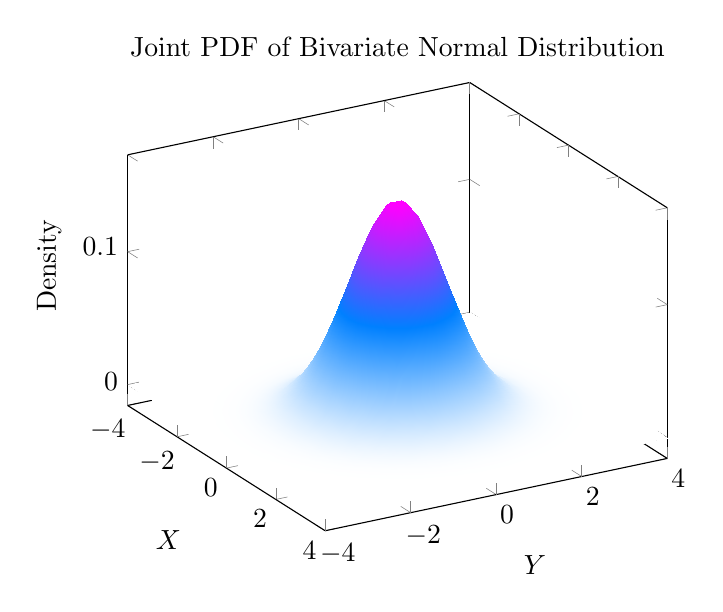
\begin{tikzpicture}
    \begin{axis}[
        xlabel={$X$},
        ylabel={$Y$},
        zlabel={Density},
        title={Joint PDF of Bivariate Normal Distribution},
        domain=-4:4,
        domain y=-4:4,
        samples=30,
        samples y=30,
        z buffer=sort,
        mesh/cols=30,
        view={60}{30},
        colormap/cool
    ]
    \addplot3[
        surf,
        shader=interp,
        samples=50,
        z buffer=sort,
        domain=-4:4,
        domain y=-4:4
    ]
    {1/(2*pi)*exp(-0.5*(x^2 + y^2))}; % Bivariate Normal PDF
    \end{axis}
\end{tikzpicture}
\end{center}

The marginal PDF can be visualized as the height of the surface obtained by fixing one variable and observing the distribution of the other. For example, the marginal PDF of \( X \) can be visualized as a 2D slice of the joint PDF along the \( X \)-axis. 
\begin{center}
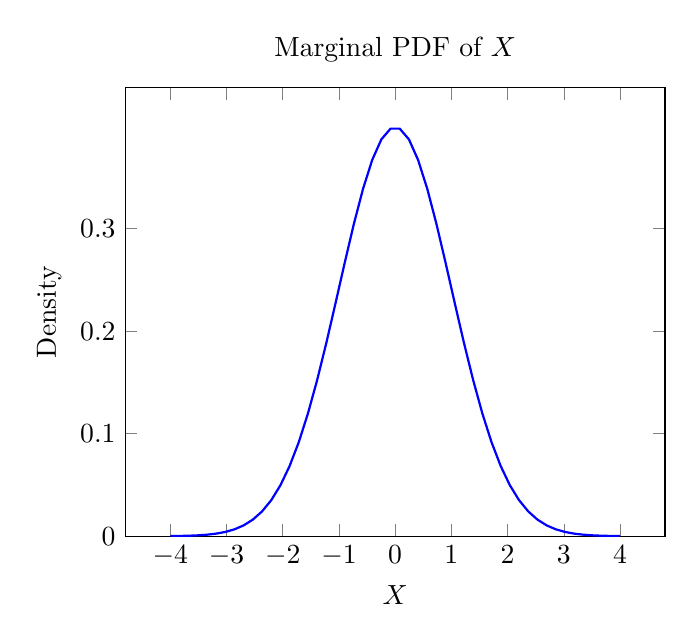
\begin{tikzpicture}
    \begin{axis}[
        xlabel={$X$},
        ylabel={Density},
        title={Marginal PDF of $X$},
        domain=-4:4,
        samples=50,
        ymin=0,
        ytick={0,0.1,0.2,0.3},
        xtick={-4,-3,-2,-1,0,1,2,3,4}
    ]
    \addplot[blue, thick] {1/sqrt(2*pi)*exp(-0.5*x^2)};
    \end{axis}
\end{tikzpicture}
\end{center}

Remember, for conditional probability, we take a vertical slice of the joint PDF corresponding to the observed value of \( X \); since the total area under this slice is \( f_X(x) \), we then divide by \( f_X(x) \) to ensure that the conditional PDF will have an area of 1.

\begin{center}
    \begin{tikzpicture}[scale=0.8]
        % 3D Normal distribution
        \begin{axis}[
            width=10cm, height=8cm,
            xlabel=$X$, ylabel=$Y$, zlabel={$f_{X,Y}(x,y)$},
            xlabel style={sloped like x axis},
            ylabel style={sloped like y axis},
            zmin=0, zmax=0.2,
            view={30}{20},
            colormap/cool
        ]
            \addplot3[
                surf,
                samples=30,
                domain=-3:3,
                y domain=-3:3,
            ] {exp(-(x^2+y^2)/2)/(2*pi)};
            
            % Vertical slice
            \addplot3[domain=-3:3, samples=30, color=red, thick] 
                ({1}, x, {exp(-(1^2+x^2)/2)/(2*pi)});
            
            % Highlight observed X value
            \draw[dashed, thick] (axis cs:1,-3,0) -- (axis cs:1,3,0);
            \node[below] at (axis cs:1,-3,0) {$x$};
        \end{axis}
        
        % Annotation for joint PDF
        \node[above] at (current axis.north east) {Joint PDF $f_{X,Y}(x,y)$};
        
        % 2D slice
        \begin{axis}[
            at={($(current axis.east)+(3cm,0)$)},
            anchor=west,
            width=6cm, height=8cm,
            xlabel=$Y$, ylabel={$f_{Y|X}(y|x)$},
            title={Conditional PDF},
            ymin=0, ymax=0.5,
        ]
            \addplot[domain=-3:3, samples=100, thick, color=red] 
                {exp(-x^2/2)/sqrt(2*pi)};
            \addplot[domain=-3:3, samples=100, dashed] 
                {0.5*exp(-x^2/2)/sqrt(2*pi)};
            \node at (axis cs:2.5,0.45) {$\frac{f_{X,Y}(x,y)}{f_X(x)}$};
            \node[color=red] at (axis cs:-2.5,0.35) {Normalized};
        \end{axis}
    \end{tikzpicture}
    \end{center}

\subsection{Independence of Random Variables}

Two random variables \( X \) and \( Y \) are said to be \textit{independent} if the occurrence of one does not affect the probability distribution of the other. This concept can be formally defined in terms of their joint and marginal probability mass functions (PMFs).

\begin{definition}
    The random variables \( X \) and \( Y \) are independent if and only if the following condition holds for all \( x \) and \( y \):

\[
P(X = x, Y = y) = P(X = x) P(Y = y).
\]

\end{definition}

This means that the joint PMF of \( X \) and \( Y \) can be expressed as the product of their marginal PMFs.

\subsubsection{Equivalent Conditions}

The independence of random variables can also be expressed in several equivalent forms:\\

1. \textbf{For all Events}: \( X \) and \( Y \) are independent if for any two events \( A \) and \( B \),
   \[
   P(A \cap B) = P(A) P(B).
   \]

2. \textbf{In terms of Expectations}: If \( X \) and \( Y \) are independent, then for any functions \( g \) and \( h \),
   \[
   E[g(X) h(Y)] = E[g(X)] E[h(Y)].
   \]

\begin{example}
    Consider two dice rolls \( X \) and \( Y \), where \( X \) represents the outcome of the first die and \( Y \) represents the outcome of the second die. Since the outcome of one die does not affect the outcome of the other, we can show their independence.\\

The joint PMF is given by:
\[
P(X = x, Y = y) = \frac{1}{36} \quad \text{for } x, y \in \{1, 2, \ldots, 6\}.
\]

The marginal PMFs are:
\[
P(X = x) = \frac{1}{6} \quad \text{and} \quad P(Y = y) = \frac{1}{6}.
\]

Verifying independence:
\[
P(X = x, Y = y) = \frac{1}{36} = P(X = x) P(Y = y) = \left(\frac{1}{6}\right)\left(\frac{1}{6}\right) = \frac{1}{36}.
\]

Thus, \( X \) and \( Y \) are independent random variables.
\end{example}

\begin{example}
    Consider two independent continuous random variables \( X \) and \( Y \) with the following PDFs:

\[
f_X(x) = \begin{cases} 
\frac{1}{2} & \text{for } 0 < x < 2 \\
0 & \text{otherwise}
\end{cases}, \quad
f_Y(y) = \begin{cases} 
\frac{1}{3} & \text{for } 0 < y < 3 \\
0 & \text{otherwise}
\end{cases}.
\]

The joint PDF of \( X \) and \( Y \) is:

\[
f_{X,Y}(x,y) = f_X(x) \cdot f_Y(y) = \begin{cases} 
\frac{1}{6} & \text{for } 0 < x < 2 \text{ and } 0 < y < 3 \\
0 & \text{otherwise}
\end{cases}.
\]

This demonstrates that \( X \) and \( Y \) are independent, as the joint PDF is indeed the product of the marginal PDFs.
\end{example}

\subsection{Covariance and Correlation}

\begin{definition}
    The covariance of two random variables \(X\) and \(Y\) is a measure of the degree to which the two variables change together. It is defined mathematically as:

\[
\text{Cov}(X, Y) = E\left[(X - E[X])(Y - E[Y])\right] = E[XY] - E[X]E[Y],
\]

where \(E[X]\) and \(E[Y]\) are the expected values (means) of \(X\) and \(Y\), respectively.
\end{definition}

\textbf{Interpretation}:

\begin{itemize}
    \item If \(\text{Cov}(X, Y) > 0\): \(X\) and \(Y\) tend to increase together.
    \item If \(\text{Cov}(X, Y) < 0\): When \(X\) increases, \(Y\) tends to decrease, and vice versa.
    \item If \(\text{Cov}(X, Y) = 0\): There is no linear relationship between \(X\) and \(Y\).
\end{itemize}

\begin{figure}[h]
    \centering
    \begin{tikzpicture}[scale=0.7]
        % Positive Correlation
        \begin{axis}[
            at={(0,0)},
            width=6cm, height=6cm,
            xlabel=$X$, ylabel=$Y$,
            title={Positive Correlation},
            xtick=\empty, ytick=\empty,
            xmin=-1, xmax=11, ymin=-1, ymax=11,
        ]
            \addplot[only marks, mark=*, mark size=1.5pt, color=blue] 
                coordinates {
                    (1,1.5) (2,2.2) (3,3.1) (4,3.8) (5,4.5)
                    (6,5.7) (7,6.4) (8,7.2) (9,8.1) (10,9.3)
                };
        \end{axis}
        
        % Negative Correlation
        \begin{axis}[
            at={(7cm,0)},
            width=6cm, height=6cm,
            xlabel=$X$, ylabel=$Y$,
            title={Negative Correlation},
            xtick=\empty, ytick=\empty,
            xmin=-1, xmax=11, ymin=-1, ymax=11,
        ]
            \addplot[only marks, mark=*, mark size=1.5pt, color=red] 
                coordinates {
                    (1,9.5) (2,8.8) (3,7.9) (4,7.2) (5,6.5)
                    (6,5.3) (7,4.6) (8,3.8) (9,2.9) (10,1.7)
                };
        \end{axis}
        
        % No Correlation
        \begin{axis}[
            at={(14cm,0)},
            width=6cm, height=6cm,
            xlabel=$X$, ylabel=$Y$,
            title={No Correlation},
            xtick=\empty, ytick=\empty,
            xmin=-1, xmax=11, ymin=-1, ymax=11,
        ]
            \addplot[only marks, mark=*, mark size=1.5pt, color=green!50!black] 
                coordinates {
                    (1,5.5) (2,3.2) (3,8.1) (4,2.8) (5,9.5)
                    (6,1.7) (7,6.4) (8,4.2) (9,7.1) (10,5.3)
                };
        \end{axis}
    \end{tikzpicture}
\end{figure}

\begin{example}
    Consider two random variables \(X\) and \(Y\) with the following joint distribution:

\[
\begin{array}{c|cccc}
X \backslash Y & 1 & 2 & 3 \\
\hline
1 & 0.1 & 0.2 & 0.1 \\
2 & 0.2 & 0.1 & 0.1 \\
3 & 0.1 & 0.1 & 0.1 \\
\end{array}
\]

First, we calculate the marginal distributions:

\[
P(X = 1) = 0.4, \quad P(X = 2) = 0.4, \quad P(X = 3) = 0.2,
\]
\[
P(Y = 1) = 0.4, \quad P(Y = 2) = 0.4, \quad P(Y = 3) = 0.2.
\]

Next, we calculate the expected values:

\[
E[X] = 1 \cdot 0.4 + 2 \cdot 0.4 + 3 \cdot 0.2 = 1.8,
\]
\[
E[Y] = 1 \cdot 0.4 + 2 \cdot 0.4 + 3 \cdot 0.2 = 1.8.
\]

Next, we calculate \(E[XY]\):

\[
E[XY] = 1\cdot1 \cdot 0.1 + 1\cdot2 \cdot 0.2 + 1\cdot3 \cdot 0.1 + 2\cdot1 \cdot 0.2 + 2\cdot2 \cdot 0.1 + 2\cdot3 \cdot 0.1 + 
\]
\[
    3\cdot1 \cdot 0.1 + 3\cdot2 \cdot 0.1 + 3\cdot3 \cdot 0.1 = 1.4.
\]

Now we calculate the covariance:

\[
\text{Cov}(X, Y) = E[XY] - E[X]E[Y] = 1.4 - (1.8 \cdot 1.8) = 1.4 - 3.24 = -1.84.
\]

This negative covariance indicates that \(X\) and \(Y\) tend to move in opposite directions.
\end{example}

\subsubsection{Properties of Covariance}

1. Symmetry: 
   \[
   \text{Cov}(X, Y) = \text{Cov}(Y, X).
   \]

2. Linearity: For any constants \(a\) and \(b\),
   \[
   \text{Cov}(aX + b, Y) = a \cdot \text{Cov}(X, Y).
   \]

3. Independence: If \(X\) and \(Y\) are independent, then:
   \[
   \text{Cov}(X, Y) = 0.
   \]

4. Variance Relation: The covariance of a random variable with itself is its variance:
   \[
   \text{Cov}(X, X) = \text{Var}(X).
   \]

\begin{definition}
    The correlation between two random variables \( X \) and \( Y \) is a measure of the strength and direction of their linear relationship. It is defined mathematically as:

\[
\rho(X, Y) = \frac{\text{Cov}(X, Y)}{\sigma_X \sigma_Y}
\]

where \( \text{Cov}(X, Y) \) is the covariance between \( X \) and \( Y \), and \( \sigma_X \) and \( \sigma_Y \) are the standard deviations of \( X \) and \( Y \), respectively. The correlation coefficient \( \rho(X, Y) \) ranges from -1 to 1.
\end{definition}

\textbf{Difference between Covariance and Correlation:}\\

Covariance provides information about the direction of the relationship but is affected by the scale of the variables. Correlation standardizes this relationship, making it easier to interpret the strength and direction of the relationship without the influence of scale.
\section{Some Inequalities and Limit Theorems}


\section{Markov Chains and Monte Carlo}
\section{The Bertnard's Paradox}

\vspace{10pt}
\hrule